\documentclass[english,letter paper,12pt,leqno]{article}
\usepackage{array}
\usepackage{stmaryrd}
\usepackage{bussproofs}
\usepackage{varwidth}
\usepackage{amsmath, amscd, amssymb, mathrsfs, accents, amsfonts,amsthm}
\usepackage[all]{xy}
\usepackage{mathtools}
\usepackage{dsfont}
\usepackage{tikz}
\def\nicedashedcolourscheme{\shadedraw[top color=blue!22, bottom color=blue!22, draw=gray, dashed]}
\def\nicecolourscheme{\shadedraw[top color=blue!22, bottom color=blue!22, draw=white]}
\def\nicepalecolourscheme{\shadedraw[top color=blue!12, bottom color=blue!12, draw=white]}
\def\nicenocolourscheme{\shadedraw[top color=gray!2, bottom color=gray!25, draw=white]}
\def\nicereallynocolourscheme{\shadedraw[top color=white!2, bottom color=white!25, draw=white]}
\definecolor{Myblue}{rgb}{0,0,0.6}
\usepackage[a4paper,colorlinks,citecolor=Myblue,linkcolor=Myblue,urlcolor=Myblue,pdfpagemode=None]{hyperref}

\SelectTips{cm}{}

\setlength{\evensidemargin}{0.1in}
\setlength{\oddsidemargin}{0.1in}
\setlength{\textwidth}{6.3in}
\setlength{\topmargin}{0.0in}
\setlength{\textheight}{8.5in}
\setlength{\headheight}{0in}

\newtheorem{theorem}{Theorem}[section]
\newtheorem{proposition}[theorem]{Proposition}
\newtheorem{lemma}[theorem]{Lemma}
\newtheorem{corollary}[theorem]{Corollary}
\newtheorem{setup}[theorem]{Setup}

% Labels in tabular
\newcommand{\tagarray}{\mbox{}\refstepcounter{equation}$(\theequation)$}

\newenvironment{mathprooftree}
  {\varwidth{.9\textwidth}\centering\leavevmode}
  {\DisplayProof\endvarwidth}
  
\newtheoremstyle{example}{\topsep}{\topsep}
	{}
	{}
	{\bfseries}
	{.}
	{2pt}
	{\thmname{#1}\thmnumber{ #2}\thmnote{ #3}}
	
	\theoremstyle{example}
	\newtheorem{definition}[theorem]{Definition}
	\newtheorem{example}[theorem]{Example}
	\newtheorem{remark}[theorem]{Remark}
	\newtheorem{strat}[theorem]{Strategy}

\numberwithin{equation}{section}

% Operators
\def\eval{\operatorname{ev}}
\def\res{\operatorname{Res}}
\def\Coker{\operatorname{Coker}}
\def\Ker{\operatorname{Ker}}
\def\im{\operatorname{Im}}
\def\can{\operatorname{can}}
\def\K{\mathbf{K}}
\def\D{\mathbf{D}}
\def\N{\mathbf{N}}
\def\LG{\mathcal{LG}}
\def\Ab{\operatorname{Ab}}
\def\stab{\operatorname{stab}}
\def\Hom{\operatorname{Hom}}
\def\Func{\operatorname{Func}}
\def\modd{\operatorname{mod}}
\def\Modd{\operatorname{Mod}}
\def\be{\begin{equation}}
\def\ee{\end{equation}}
\def\nN{\mathds{N}}
\def\nZ{\mathds{Z}}
\def\nQ{\mathds{Q}}
\def\nR{\mathds{R}}
\def\nC{\mathds{C}}
\DeclareMathOperator{\Ext}{Ext}
\DeclareMathOperator{\Tr}{Tr}
\DeclareMathOperator{\End}{End}
\DeclareMathOperator{\rank}{rank}
\DeclareMathOperator{\tot}{Tot}
\DeclareMathOperator{\ch}{ch}
\DeclareMathOperator{\str}{str}
\DeclareMathOperator{\hmf}{hmf}
\DeclareMathOperator{\HMF}{HMF}
\DeclareMathOperator{\hf}{HF}
\DeclareMathOperator{\At}{At}
\DeclareMathOperator{\Cat}{Cat}
\DeclareMathOperator{\Spec}{Spec}
\DeclareMathOperator{\id}{id}
\DeclareMathOperator{\derelict}{derelict}

\begin{document}

% Commands
\def\Res{\res\!}
\newcommand{\ud}{\mathrm{d}}
\newcommand{\Ress}[1]{\res_{#1}\!}
\newcommand{\cat}[1]{\mathcal{#1}}
\newcommand{\lto}{\longrightarrow}
\newcommand{\xlto}[1]{\stackrel{#1}\lto}
\newcommand{\mf}[1]{\mathfrak{#1}}
\newcommand{\md}[1]{\mathscr{#1}}
\def\sus{\l}
\def\l{\,|\,}
\def\sgn{\textup{sgn}}
\newcommand{\den}[1]{\llbracket #1 \rrbracket}
\def\inta{\textbf{int}}
\def\binta{\textbf{bint}}
\def\comp{\underline{\textup{comp}}}
\def\mult{\underline{\textup{mult}}}
\def\repeat{\underline{\textup{repeat}}}
\def\master{\underline{\textup{master}}}

\DeclarePairedDelimiter\bra{\langle}{\rvert}
\DeclarePairedDelimiter\ket{\lvert}{\rangle}

\title{Linear logic and recurrent neural networks}
\author{Huiyi Hu, Daniel Murfet}

\maketitle

\section{Introduction}

In recent years deep neural networks have proven to be proficient at learning hierarchical vector representations of natural data, including images and language \cite{dlnature}. If we follow Leibniz \cite{frege} in believing that reasoning is the algebraic manipulation of such representations or ``symbols" then it is natural to look for systems which augment the capacity of neural networks for performing these kinds of manipulations. There are by now numerous proposals for how to achieve this, including neural Turing machines \cite{ntm}, stack-augmented recurrent neural networks \cite{joulin}, differentiable neural computers \cite{dnc} and others \cite{graves_etal, grefen, weston, tarlow}. We investigate a new approach, based on the Curry-Howard isomorphism and linear logic.

The Curry-Howard isomorphism \cite{sorensen} gives a bijection between a prototypical system of formal reasoning (Gentzen's natural deduction) and a prototypical algorithmic system (Church's simply-typed lambda calculus). For this reason the lambda calculus and derivative languages such as LISP have played an important role in the symbolic approach to reasoning in the modern field of artificial intelligence. While these methods may have been overshadowed in recent decades by the rise of the connectionist approach, now called deep learning, it has been argued that a synthesis of the two approaches is necessary to achieve general reasoning in a connectionist system \cite{minsky}. The main obstacle to this synthesis is the discrepancy between the discrete symbolic nature of natural deduction, or equivalently lambda calculus, and the differentiable nature of neural networks. One way to overcome this obstacle is to augment a neural network not directly with symbolic logic, but rather with a \emph{differentiable model} of logic; and the most natural way to construct such a model is not to work directly with simply-typed lambda calculus but rather with a refinement due to Girard known as linear logic \cite{girard} which has a canonical model (called a denotational semantics) in differentiable maps between vector spaces \cite{ehrhard-survey,blutecon,murfetclift}. 
\\

We demonstrate one concrete realisation of these ideas in the form of a Recurrent Neural Network (RNN) controller \cite{elman} augmented with spaces of linear logic programs. At each time step the controller predicts which commands (denotations of linear logic programs) to run and the inputs to run them on, from its hidden state and the current input. We call the resulting system the \emph{Linear Logic Recurrent Neural Network} or LLRNN. This architecture is inspired by many papers in the neural network literature, most notably the second-order RNN \cite{joulin} and multiplicative RNN \cite{sutskever}.

% Linear logic programs are quite general, and some existing augmentations of RNNs can be realised as special cases of the LLRNN. This is theoretically attractive as it gives a unified construction, but the main point is that the framework suggests natural extensions of these models. For example, an important subset of the memory augmentations in the Neural Turing Machine (NTM) \cite{ntm} and Differentiable Neural Computer (DNC) of \cite{dnc} can be realised as special cases of the LLRNN. Since these systems have good properties, our experiments explore extensions of the DNC which add read and write heads storing linear logic programs, which can be applied to stored vectors as a generalisation of the ``read'' operation of the DNC.

%  which predicts at time $t$ a linear combination of denotations of linear logic programs (or proofs) to be applied to vectors which are themselves predicted from the hidden state of the RNN at time $t-1$ and the input symbol at time $t$. The output of the linear logic program is a linear operator, which is applied to the hidden state at time $t-1$ to generate a vector which is then added to the usual update equation of the RNN. 



% Our approach is to augment an RNN controller with a library of functional programs using the polynomial semantics of differential linear logic \cite{murfet_ll,murfetclift}. Differential $\lambda$-calculus \cite{difflambda} and the related system of differential linear logic \cite{ehrhard-survey} may be viewed as functional programming languages in which programs naturally admit derivatives. These derivatives exist at both the syntactic and semantic level, and the differential structure of the language is what guarantees that the programs are compatible with backpropagation. The existence of this general theory demonstrates the naturality of our approach, but in the present paper the programs involved are so simple that we will not need to invoke the theory; for more details see Section \ref{section:differential_linear}.

\section{Architecture}

\subsection{The second-order RNN}

As usual we use ``weight'' as a synonym for variable, or more precisely, the variables which we will vary during gradient descent. We denote by $\sigma$ the function
\begin{gather*}
\sigma: \mathbb{R}^k \lto \mathbb{R}^k\,\\
\sigma( \bold{x} )_i = \frac{1}{2}( x_i + |x_i| )
\end{gather*}
and by $\zeta$ the \emph{softmax} function
\begin{gather*}
\zeta: \mathbb{R}^k \lto \mathbb{R}^k\,,\\
\zeta(\bold{x})_i = \frac{e^{x_i}}{\sum_{j=1}^k e^{x_j}}\,.
\end{gather*}
An RNN is defined by its \emph{evolution equation} which expresses $h^{(t+1)}$ as a function of $h^{(t)}, x^{(t)}$ and its \emph{output equation} which gives the output $y^{(t)}$ as a function of $h^{(t)}$. At time $t \ge 1$ we denote the hidden state by $h^{(t)}$ and the input by $x^{(t)}$. 

\begin{definition} A standard Elman-style RNN \cite{elman} is defined by weight matrices $H, U, B$ and the evolution equation
\be\label{eq:update_eqn}
h^{(t+1)} = \sigma\big( H h^{(t)} + U x^{(t+1)} + B\big)
\ee
where $h^{(0)}$ is some specified initial state. The outputs are defined by
\be\label{eq:output_rnn}
y^{(t)} = \sigma\big( W_y h^{(t)} + B_y \big)\,.
\ee
\end{definition}
Suppose the input vector space is $\mathscr{I}$ and the hidden state space is $\mathscr{H}$, so that $x^{(t)} \in \mathscr{I}$ and $h^{(t)} \in \mathscr{H}$ for all $t$. The value of the RNN on a sequence $\bold{x} = \big( x^{(1)}, \ldots, x^{(T)} \big) \in \mathscr{I}^{\oplus T}$ is computed by applying \eqref{eq:update_eqn} for $0 \le t \le T - 1$, accumulating the values $\bold{y} = (y^{(1)}, \ldots, y^{(T)})$ from each time step, and finally applying a fully-connected layer and the softmax function $\tau$ obtain the output sequence $o^{(t)} = \zeta( W_o y^{(t)} + B_o )$. Each $o^{(t)}$ has the property that its components in our chosen basis add to $1$. We view such a vector as a probability distribution over the basis, sampling from which gives the output of the RNN on $\bold{x}$.
\\
%Note that the evolution equation implicitly determines a piecewise-linear function
%\begin{gather*}
%\mathscr{I} \lto \operatorname{Func}(\mathscr{H}, \mathscr{H} )\,,\\
%x \mapsto \sigma\big( H (-) + U x + B\big)\,,
%\end{gather*}
%which specifies how we may view inputs as transforming the internal state of the RNN. One class of modifications of the RNN architecture adds more complicated (for example, piecewise-polynomial of higher degree) transformations of the internal state.

We consider a generalisation of the second-order RNN \cite{highorderrec,pollack,firstvsecond,secondorder} and the similar multiplicative RNN \cite{sutskever}. In addition to the hidden-to-hidden matrix $H$ and the input-to-hidden matrix $U$ of the traditional RNN, the second-order RNN learns a matrix $V$ that maps inputs to linear operators on the hidden state. More precisely, a vector is added to the evolution equation whose $i$th coordinate is given by the formula
\be\label{eq:2ndorderrnn}
\sum_j \sum_k V^{jk}_{i} h^{(t)}_j x^{(t+1)}_k
\ee
where $V$ is interpreted as a tensor in
\be\label{eq:input_to_operator}
\mathscr{I}^* \otimes \mathscr{H}^* \otimes \mathscr{H} \cong \Hom_{\mathbb{R}}(\mathscr{I} , \End_{\mathbb{R}}(\mathscr{H}))\,.
\ee
Identifying the tensor $V$ with a linear map from the input space $\mathscr{I}$ to linear operators on $\mathscr{H}$, we have that $V(x^{(t+1)})(h^{(t)})$ is the vector whose $i$th coordinate is \eqref{eq:2ndorderrnn}. 

\begin{definition} The second-order RNN \cite{highorderrec,pollack} is defined by weights $H,U,B,V$ and
\be\label{eq:second_order_evolution}
h^{(t+1)} = \sigma\big( V( x^{(t+1)} )(h^{(t)}) + H h^{(t)} + U x^{(t+1)} + B\big)\,,
\ee 
with $y^{(t)}, o^{(t)}$ as before.
\end{definition}

The problem with second-order RNNs is that they may be difficult to train if the state space is large, since $\dim(\End_{\mathbb{R}}(\mathscr{H})) = \dim(\mathscr{H})^2$. The \emph{multiplicative RNN} is introduced in \cite{sutskever} as a more tractable model. The central idea is the same, but an auxiliary space $\mathscr{K}$ is introduced and the RNN learns three linear maps
\be\label{eq:threelinearmaps}
V: \mathscr{I} \lto \End_{\mathbb{R}}(\mathscr{K})\,, \quad I: \mathscr{K} \lto \mathscr{H}\,, \quad J: \mathscr{H} \lto \mathscr{K}\,.
\ee
Moreover $V$ factors through the subspace of diagonalisable matrices in some chosen basis, so it is defined by $\dim(\mathscr{K})$ free parameters. The additional term in the evolution equation \eqref{eq:second_order_evolution} is changed to
\be\label{eq:new_term_mRNN}
I\big( V(x^{(t+1)})( J h^{(t)} ) \big)\,.
\ee
The multiplicative RNN has been applied to character-level text generation \cite{sutskever} and sentiment analysis \cite{irsoy}. This is not to be confused with the \emph{multiplicative integration} RNN of \cite{yuhai} which adds a term $H h^{(t)} \odot U x^{(t+1)}$ to the evolution equation.

\begin{remark}
The second-order RNN transforms input symbols into linear operators on its hidden state. Observe that consecutive symbols $x = x^{(t)}$ and $x' = x^{(t+1)}$ in the input become composed operators on the hidden state, since (ignoring the non-linearity)
\begin{align*}
V(x')(h^{(t)}) &= V(x')\big( V(x)(h^{(t-1)}) + \cdots)\\
&= \big\{ V(x') \circ V(x) \big\}( h^{(t-1)} ) + \cdots\,.
\end{align*}
The relevance of this ``compositionality'' to NLP is remarked on in \cite{irsoy}.
\end{remark}


\subsection{The linear logic RNN}

At each time step the second-order RNN generates from its input a linear operator which is applied to to the hidden state; this operator moreover depends \emph{linearly} on the input given to the RNN. The LLRNN model is similar to the second-order RNN in the sense that it generates at each time step a linear operator which is applied to the hidden state, but dissimilar in that this operator depends \emph{non-linearly} on the input as well as a sequence of other vectors generated from the hidden state.

The non-linear function which computes the operator to be applied to the hidden state at each time step is called the \emph{master algorithm}. It is itself the denotation of a proof in linear logic. The arguments to the master algorithm are:
\begin{itemize}
\item A sequence of \emph{command vectors} $p_i^{(t+1)}$ generated via softmax $\zeta$ from $h^{(t)}$,
\item a sequence of \emph{data vectors} $b_i^{(t+1)}$ generated via $\sigma$ from $h^{(t)}$,
\item an \emph{input vector} $c^{(t+1)}$ generated via $\sigma$ from $x^{(t+1)}$.
\end{itemize}
The idea is that the command vectors give distributions over finite-dimensional spaces of linear logic programs, while the data vectors and input vector give the inputs to be fed in some way into the selected programs; the exact details of this ``feeding'' are specified by the master algorithm itself.
\\

We refer to \cite{murfet_ll,murfetclift} for reviews of the relevant parts of linear logic, and the proof that proof denotations give smooth maps. Recall that the \emph{types} of intuitionistic linear logic are built from atomic variables via binary connectives $\otimes, \multimap$ (tensor, Hom) and a unary connective ${!}$ (called bang). The denotational semantics $\den{-}$ of linear logic in the category $\cat{V}$ of vector spaces from \cite[\S 5.1, \S 5.3]{murfet_ll} is defined as follows: for a variable $x$ the denotation $\den{x}$ is a chosen finite-dimensional vector space, and
\begin{align*}
\den{A \multimap B} &= \Hom_k(\den{A},\den{B})\,,\\
\den{A \otimes B} &= \den{A} \otimes \den{B}\,,\\
\den{{!}A} &= {!} \den{A}\,,
\end{align*}
where ${!} V$ denotes the universal cocommutative counital coalgebra mapping to $V$. Here $\Hom_{\mathbb{R}}(W,V)$ denotes the space of linear maps from $W$ to $V$ and $\End_{\mathbb{R}}(V) = \Hom_{\mathbb{R}}(V,V)$.

For any proof $\pi$ of type $A$ the denotation is a vector $\den{\pi} \in \den{A}$. Moreover to a proof $\pi$ of type ${!} A \multimap B$ we naturally associate \cite[Definition 5.10]{murfet_ll} a function $\den{\pi}_{nl}: \den{A} \lto \den{B}$.

\begin{definition} The Linear Logic Recurrent Neural Network (LLRNN) is determined by the following data:
\begin{itemize}
\item types $P_1,\ldots,P_r$ called the \emph{command types};
\item types $B_1,\ldots,B_s$, called the \emph{data types};
\item a type $C$, called the \emph{input type};
\item a type $A$ with $\den{A} = \mathscr{H}$, the hidden state space;
\item two proofs $\underline{\mathrm{master}}^z$ for $z \in \{\mathrm{in},\mathrm{out}\}$ of the sequent
\be
{!} P_1, \ldots, \, {!}P_r,\, {!} B_1, \ldots,\, {!} B_s,\, {!} C \vdash A \multimap A\,.
\ee
\item Finite-dimensional subspaces for $1 \le i \le r$ and $1 \le j \le s$
\be
\mathscr{P}_i \subseteq \den{P_i}\,, \quad \mathscr{B}_j \subseteq \den{B_j}\,, \quad \mathscr{C} \subseteq \den{C}
\ee
which are spanned by the denotations of linear logic proofs. We refer to the elements of $\mathscr{P}_i$ as \emph{command vectors}, elements of $\mathscr{B}_j$ as \emph{data vectors} and elements of $\mathscr{C}$ as \emph{input vectors}.
\end{itemize}
\end{definition}
From this data we obtain the following functions by restriction:
\be
\den{\underline{\mathrm{master}}^z}_{nl}: \mathscr{P}_1 \times \cdots \times \mathscr{P}_r \times \mathscr{B}_1 \times \cdots \times \mathscr{B}_s \times \mathscr{C} \lto \End_{\mathbb{R}}(\mathscr{H})\,.
\ee
The coupling of the master algorithm to the RNN controller is given by
\begin{align*}
p_i^{(t+1)} &= \zeta( W^p_i h^{(t)} + B^p_i ) \in \mathscr{P}_i\,, \qquad 1 \le i \le r\,,\\
b_j^{(t+1)} &= \sigma( W^b_j h^{(t)} + B^b_j ) \in \mathscr{B}_j\,, \qquad 1 \le j \le s\,,\\
c^{(t+1)} &=  W^c x^{(t+1)} \in \mathscr{C}
\end{align*}
and the evolution equation
\be\label{eq:masterh}
h^{(t+1)} = \sigma\Big( Z_{\mathrm{in}} + H h^{(t)} + U x^{(t+1)} + B\Big) + Z_{\mathrm{out}}
\ee
where the new term $Z$, is for $z \in \{\mathrm{in},\mathrm{out}\}$,
\be\label{eq:masterz}
Z_z = \den{\underline{\mathrm{master}}^z}_{nl}\Big( p_1^{(t+1)}, \ldots, p_r^{(t+1)}, b_1^{(t+1)}, \ldots, b_s^{(t+1)}, c^{(t+1)}\Big)(h^{(t)})\,.
\ee

The fundamental fact which makes this model reasonable is the following:

\begin{proposition} The functions $\den{\master^z}_{nl}$ are smooth.
\end{proposition}
\begin{proof}
This follows from the hypothesis that $\mathscr{P}_i, \mathscr{B}_j$ are generated by denotations of linear logic proofs, and the smoothness of these denotations \cite{murfetclift}.
\end{proof}

Moreover, the derivatives of $\den{\master^z}_{nl}$ can be computed symbolically using the cut-elimination algorithm of differential linear logic, and it is therefore feasible to implement a general LLRNN in a software package like TensorFlow. 

\begin{remark}\label{remark:sequentbang} It will often be convenient to write $\Gamma = P_1, \ldots, P_r$ for the command types and $\Delta = B_1, \ldots, B_s$ for the data types. A standard notational device in the linear logic literature is to then write ${!} \Gamma$ for the list preprending ${!}$ to all the types in the list $\Gamma$, that is, ${!} \Gamma = {!} P_1, \ldots, {!} P_r$. With this notation, $\master$ is a proof of ${!} \Gamma, {!} \Delta, {!} V \vdash A \multimap A$.
\end{remark}

\section{Examples of the LLRNN}

As defined the LLRNN is a class of models. In this section we explain how to implement various existing augmentations of RNNs, including a subset of the Neural Turing Machine, in the framework of the LLRNN. The guiding intuition from logic is that the complexity of an algorithm is rooted in the kind of \emph{iteration} that it employs; for an exposition in the context of linear logic see \cite[\S 7]{murfet_ll}. From this point of view, the purpose of augmenting an RNN with linear logic is to provide access to iterators of a complexity ``similar'' to the function that the neural network is trying to approximate.

The most elementary form of iteration is repetition. The simplest example of this form of iteration in the current context is raising a linear operator to an integer power. This non-linear transformation of an input operator $\alpha \in \End_{\mathbb{R}}(\mathscr{H})$ to the output operator $\alpha^n$ is encoded by a proof $\underline{n}$ in linear logic of the type
\[
\textbf{int}_A = {!}(A \multimap A) \multimap (A \multimap A)
\]
where $\den{A} = \mathscr{H}$. A more interesting kind of iteration takes a pair of linear operators $\alpha, \beta$ and intertwines them according to a sequence of binary numbers $S \in \{0,1\}^*$. This transformation is encoded by a proof $\underline{S}$ in linear logic of type
\[
\textbf{bint}_A = {!}(A \multimap A) \multimap \big({!}(A \multimap A) \multimap (A \multimap A)\big)\,.
\]
We begin this section with a brief exposition on the iterators $\underline{n}$ and $\underline{S}$ before going on to explain how they appear in various special cases of the LLRNN. The iterator $\underline{n}$ is the basic tool in the linear logic implementation of the NTM (Section \ref{example:ntm}) and its generalisations in Section \ref{example:ntm_extended} and Section \ref{example:ntm_super} while the iterator $\underline{S}$ is used in Example \ref{example:dihedral}. 

The reader may prefer to substitute \emph{program} wherever we write \emph{proof} in what follows, following Curry-Howard \cite{sorensen}. There are two ways of presenting proofs in linear logic: proof trees, and the term calculus of \cite{benton_etal} which is a refinement of the lambda calculus, and we will use the latter in the following examples.
\vspace{0.25cm}

For more details on the following examples from linear logic see \cite[\S 3]{murfetclift}. 

\begin{example}\label{example_1} The denotation of a proof $\pi$ of type $\textbf{int}_A$ is a function
\[
\den{\pi}_{nl}: \End_{\mathbb{R}}(\den{A}) \lto \End_{\mathbb{R}}(\den{A})
\]
which is a polynomial function of the entries of the input matrix. For each integer $n \ge 0$ there is a proof $\underline{n}$ of type $\inta_A$. For example, in the term calculus of \cite{benton_etal}
\[
\underline{2} = (\lambda q.(\textrm{copy $q$ as $h,g$ in } (\lambda z. (\derelict(g) \; (\derelict(h)\; z)))\,.
\]
The denotation satisfies $\den{\underline{n}}_{nl}(X) = X^n$. %To be clear, writing $\mathscr{K} = \mathbb{R}^{n_H}$ and identifying $\End_{\mathbb{R}}(\mathscr{K})$ with the space of matrices $M_{n_H}(\mathbb{R})$, the denotation of any proof of $\textbf{int}_\alpha$ will be a function $\den{\pi}(X)_{ij}: M_{n_H}(\mathbb{R}) \lto \mathbb{R}$ which is a polynomial in the entries $X_{kl}$ for $1 \le i, j \le n_H$.
\end{example}

\begin{example}\label{example_2} The denotation of a proof $\pi$ of type $\textbf{bint}_A$ is a polynomial function
\[
\den{\pi}_{nl}: \End_{\mathbb{R}}(\den{A}) \times \End_{\mathbb{R}}(\den{A}) \lto \End_{\mathbb{R}}(\den{A})\,.
\]
For every binary sequence $S \in \{0,1\}^*$ there is a corresponding proof $\underline{S}$ of $\binta_A$ \cite[\S 3.2]{murfetclift}, with for example
\[
\underline{001} = (\lambda q.(\lambda p.(\textrm{copy $q$ as $r,s$ in } (\lambda z.(\derelict(p)\;(\derelict(s)\;(\derelict(r)\;z)))))))\,.
\]
The denotation $\den{\underline{S}}$ sends a pair of matrices $X,Y$ to the product described by $S$, reading $X$ for $0$ and $Y$ for $1$, and reading in reverse order. For example,
\[
\den{\underline{001}}(X,Y) = Y X X\,.
\]
\end{example}

\begin{example}[(Second-order RNN)] With $r = s = 0$ there are no command or data vectors. Take for the input type $C = A \multimap A$ and
\[
\mathscr{C} = \End_{\mathbb{R}}(\mathscr{H}) = \den{A \multimap A}\,.
\]
so the master algorithm takes a single input, which is a linear operator on the hidden state, and returns such an operator. The only weight matrix involved in the LLRNN beyond the usual RNN is the matrix $W^c$ which maps inputs to linear operators on $\mathscr{H}$.

We choose $\master^{\mathrm{in}}$ to be the proof of ${!}(A \multimap A) \vdash A \multimap A$ which is given by dereliction, so that $\den{\master^{\mathrm{in}}}_{nl}(\alpha) = \alpha$ and hence
\be\label{eq:secondorderRNNinLLRNN}
Z_{\mathrm{in}} = W^c(x^{(t+1)})(h^{(t)})\,.
\ee
Thus the LLRNN with these settings is just the second-order RNN.
\end{example}

The most elementary coupling of an RNN to linear logic adds the ability to raise linear operators (generated say from an input symbol, in the manner of the second-order RNN) to a power generated from the hidden state of the RNN. 

\begin{example}[(Higher-order RNN)] Consider the generalisation of the second-order RNN where the controller predicts at each time step an integer power of the linear operator $W^c(x^{(t+1)})$ to apply to the hidden state. Suppose we allow powers in the range $\{0,\ldots,L\}$. Then at each time step the RNN will generate a distribution $p^{(t+1)}$ over $\{0,\ldots,L\}$ from the current hidden state $h^{(t)}$ by the formula
\[
p^{(t+1)} = \zeta( W_p h^{(t)} + B_p )
\]
and the evolution equation is
\be\label{eq:higherorderRNN}
Z = \sum_{i=0}^L p_i^{(t+1)} \big( W^c(x^{(t+1)}) \big)^i(h^{(t)})\,.
\ee
The operation of taking a linear operator and raising it to the $n$th power is encoded by the proof $\underline{n}$ of type $\inta_A$. We can therefore represent the higher-order RNN as a LLRNN, as follows. There is one command type $\inta_A$, no data types, and input type $A \multimap A$. The spaces of command and input vectors are respectively
\begin{align*}
\mathscr{P}_1 &= \operatorname{span}(\den{\underline{0}}, \ldots, \den{\underline{L}}) \subseteq \den{\inta_A}\,,\\
\mathscr{C} &= \End_{\mathbb{R}}(\mathscr{H}) = \den{A \multimap A}\,.
\end{align*}
We omit $\master^{\mathrm{out}}$ and write $\master$ for $\master^{\mathrm{in}}$ which we take to be the proof of
\[
{!}\inta_A, \, {!}(A \multimap A) \vdash A \multimap A
\]
given in the term calculus of \cite{benton_etal} by
\[
\master = (\lambda n. (\lambda a. (\derelict(n) \; a)))\,.
\]
This proof has the property that for $n_i \ge 0$ and $\alpha \in \End_{\mathbb{R}}(\mathscr{H})$ and $p_i \in \mathbb{R}$,
\be
\den{\master}_{nl}\big( \sum_i \lambda_i \den{\underline{n}_i}, \alpha \big) = \sum_i \lambda_i \alpha^{n_i}\,.
\ee
The coupling of this function to the RNN is via $p_1^{(t+1)}$ which we identify with $p^{(t+1)}$ above, and $c^{(t+1)} = W^c(x^{(t+1)})$. By construction the LLRNN with this configuration reproduces the $Z$ of \eqref{eq:higherorderRNN} and thus the higher-order RNN.
\end{example}

Since one doesn't need to know linear logic to understand how to raise a linear operator to an integer power, it is natural to wonder to what degree linear logic is actually necessary here. All of our models can be formulated without any mention of linear logic, and indeed we will generally present the functions $\den{\master}_{nl}$ rather than the underlying proof, which we relegate to Appendix \ref{section:lambda_terms}. Nonetheless, the construction of $\master$ within linear logic constrains the model and makes conceptually clear the computational ideas involved; these ideas are not necessarily clear from the polynomial algebra that results from applying the denotation functor $\den{-}$. The strongest example of this point of view is the role of iteration in the LLRNN approach to the Neural Turing Machine and its generalisations.

\subsection{Neural Turing Machine}\label{example:ntm}

The raising of a linear operator to a power predicted from the hidden state is the crucial architectural feature behind the Neural Turing Machine (NTM) \cite{ntm} and stack-augmented RNN \cite{joulin}. The linear operator in the former case rotates the memory state, viewed as a sequence of vectors arranged at the vertices of a regular polygon. The read and write address weightings of the NTM are then controlled by predicting a distribution, at each time step, over the distinct powers of this rotation matrix. 

To explain, we introduce the \emph{address space}
\[
\mathscr{W} = (\mathbb{Z}/N\mathbb{Z})^{\mathbb{R}} \cong \mathbb{R} \bar{0} \oplus \cdots \oplus \mathbb{R} \overline{N-1}
\]
and given a \emph{memory coefficient space} $\mathscr{V}$ the \emph{memory space} is the tensor product
\[
\mathscr{S} = \mathscr{W}^* \otimes \mathscr{V} \cong \Hom_{\mathbb{R}}(\mathscr{W}, \mathscr{V})\,.
\]
A memory state $M$ is a linear map $M: \mathscr{W} \lto \mathscr{V}$ which we view as an arrangement of the vectors $u_j = M(\bar{j})$ on the vertices of the regular $N$-gon:
\begin{center}
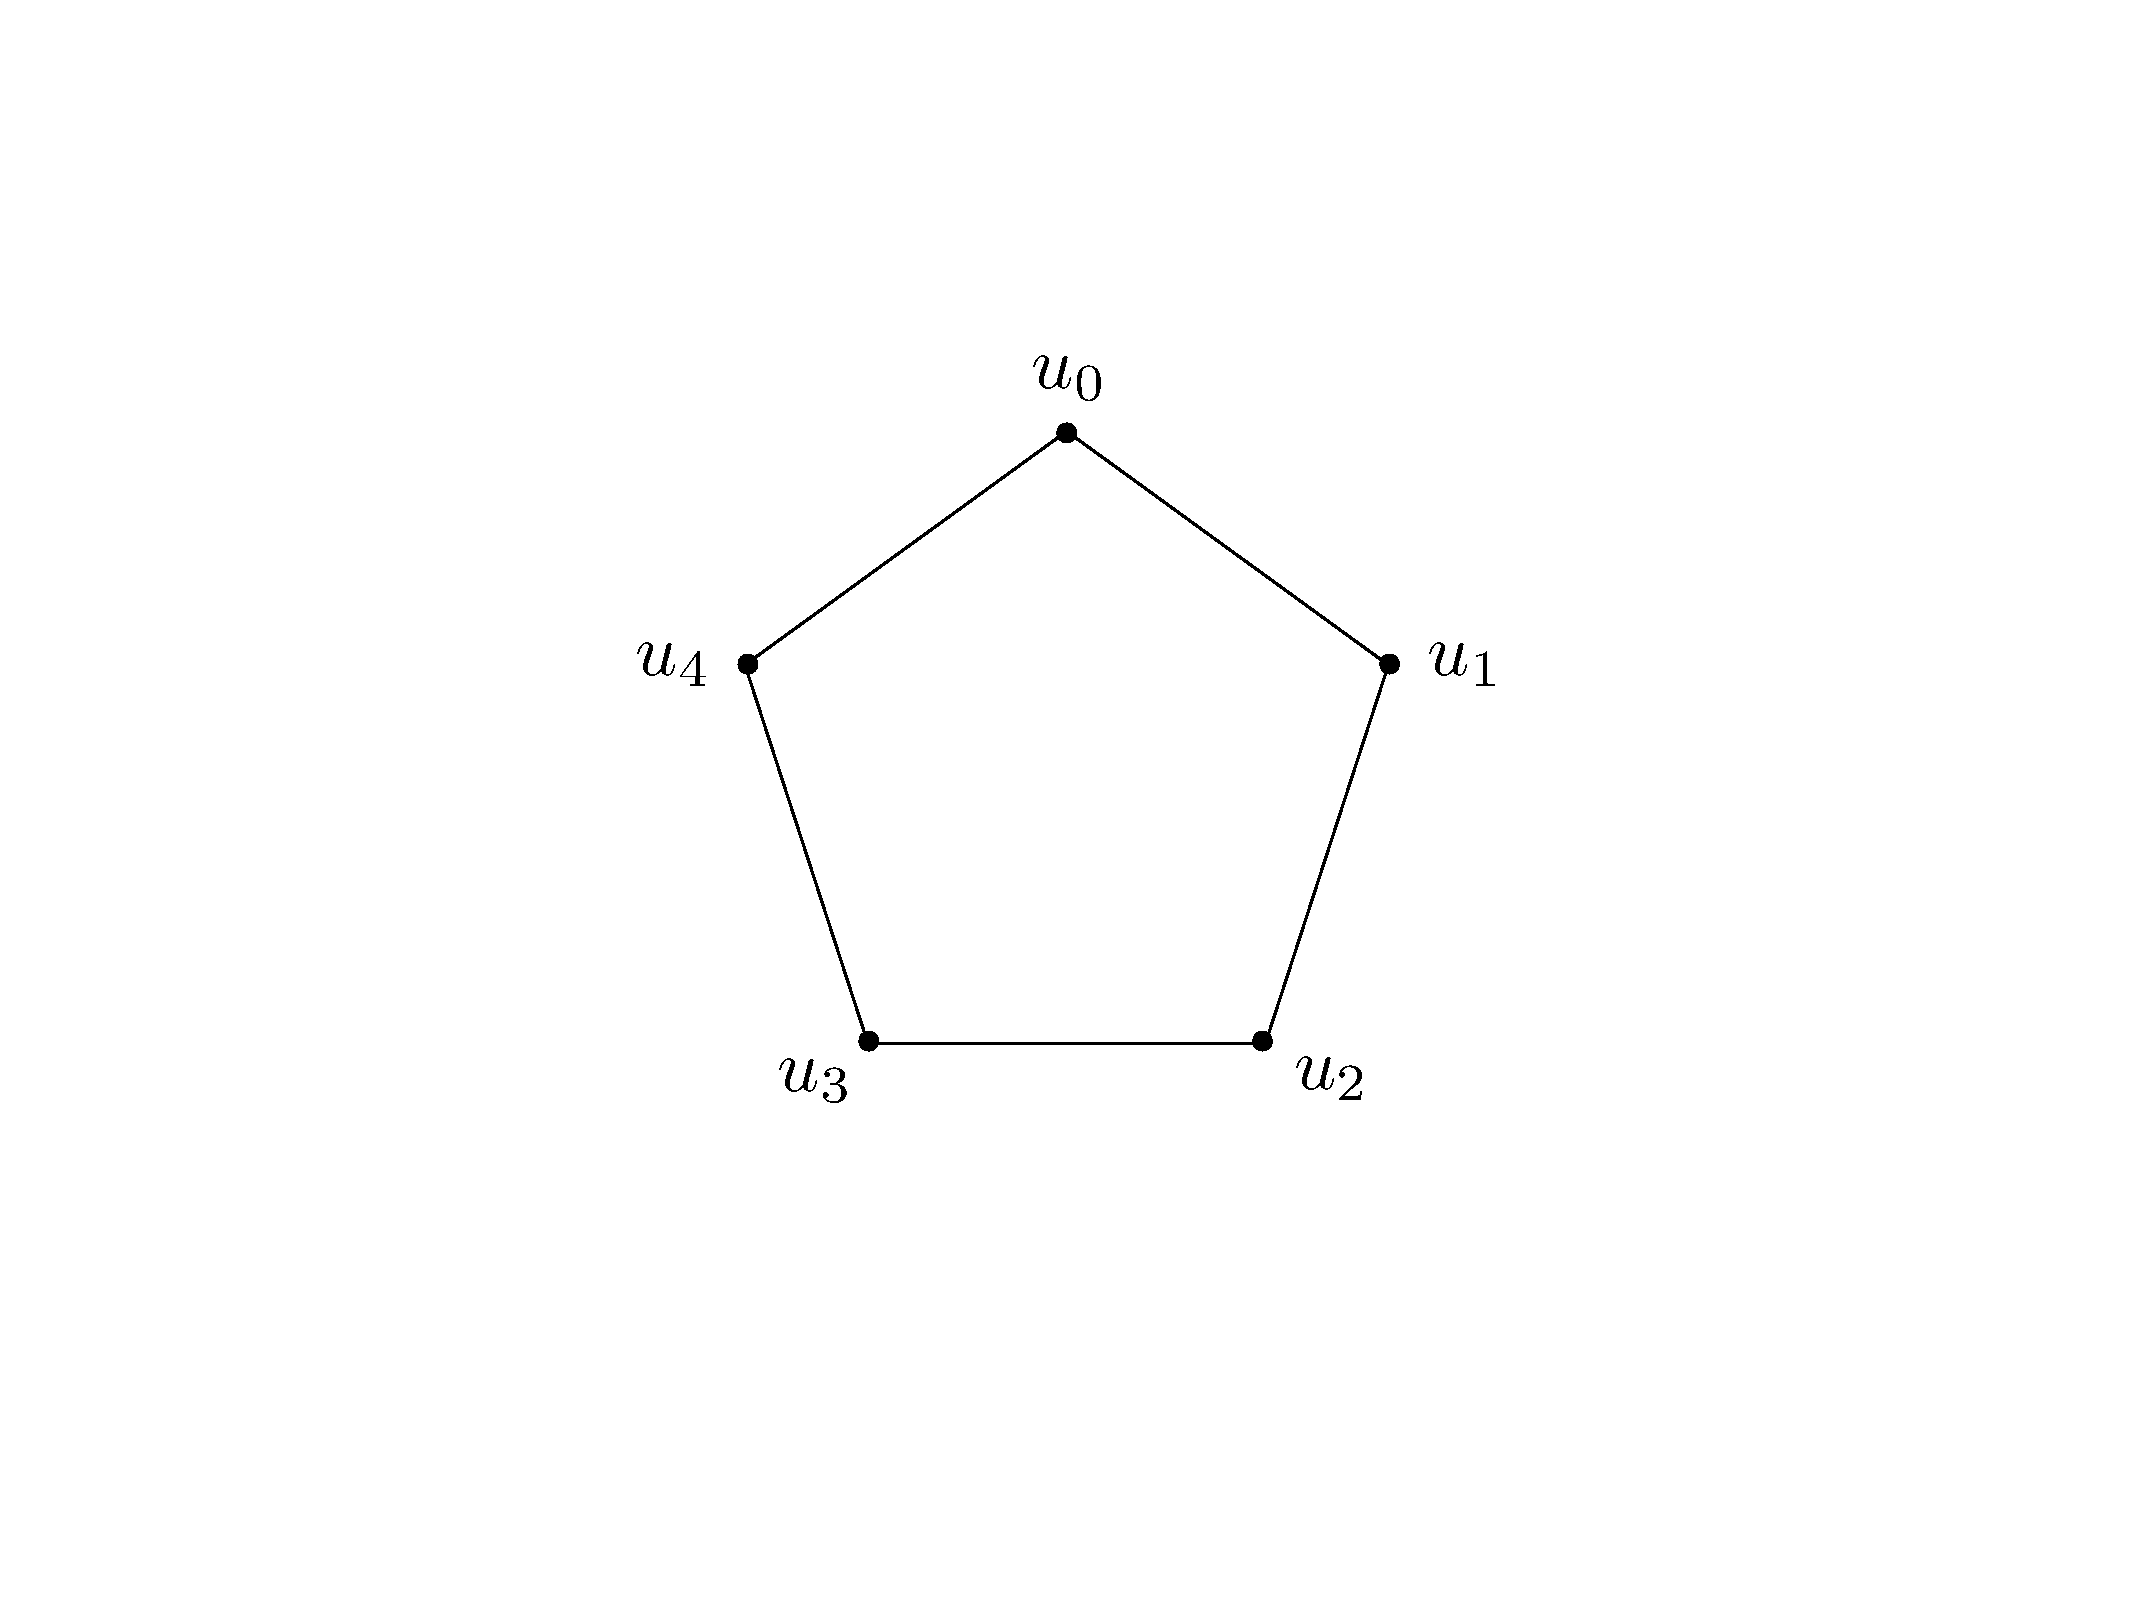
\includegraphics[scale=0.3]{dia1}
\end{center}
Sometimes we refer to this structure as a \emph{memory ring}. In the notation of \cite{ntm} we may take $\mathscr{W} = \mathbb{R}^N$ and $\mathscr{V} = \mathbb{R}^M$ so that elements of $\mathscr{S}$ are identified with $N \times M$ matrices. 

The space of memory states has a natural action of the cyclic group of order $N$, which acts by rotation on $\mathscr{W}$ and therefore on $\mathscr{S}$. The rotated state assigns the vector $u_{j+1}$ to the position $j$ (we index the positions in the clockwise order) with $j + 1$ computed modulo $N$. Said differently, let $R: \mathscr{W} \lto \mathscr{W}$ be the linear map defined by
\[
R( \overline{a} ) = \overline{a+1}\,,
\]
with dual map $R^*: \mathscr{W}^* \lto \mathscr{W}^*$. The rotation of the memory state $M$ is the composition $M \circ R$, or what is the same thing, $R^*( M )$. Thus, applying the $j$-th power of $R^*$ to a memory state has the effect of rotating the state $j$ times around the regular polygon.

The internal state space of the RNN underlying the NTM is decomposed as
\be\label{eq:decomp}
\mathscr{H} = \mathscr{H}_0 \oplus \mathscr{W} \oplus \mathscr{W}^* \oplus \mathscr{S}
\ee
and the state at time $t$ is written
\[
h^{(t)} = (h_0^{(t)}, r^{(t)}, w^{(t)}, M^{(t)}) \in \mathscr{H}\,.
\]
The components of this vector are interpreted as the \emph{controller internal state} $h_0^{(t)}$, \emph{read address weights} $r^{(t)}$, \emph{write address weights} $w^{(t)}$ and \emph{memory contents} $M^{(t)}$. For convenience we will refer to the read address weight as the \emph{read address}, even though the vector represents a distribution over the available addresses rather than a specific address. At each time step the RNN generates from its hidden state a distribution $s$ over rotations of the write address, a distribution $q$ over rotations of the read address, and a vector $u$ to be written to memory, via the formulas
\begin{gather*}
s^{(t+1)} = \zeta( W_s h^{(t)} + B_s ) \in \mathscr{W}^*\,,\\
q^{(t+1)} = \zeta( W_q h^{(t)} + B_q ) \in \mathscr{W}^*\,,\\
u^{(t+1)} = \sigma( W_a h^{(t)} + B_a ) - \sigma( W_e h^{(t)} + B_e ) \in \mathscr{V}\,.
\end{gather*}
The update equation for the addresses \cite[Eq. (8)]{ntm} and memory \cite[Eq. (3),(4)]{ntm} are
\begin{align}
w^{(t+1)} = \sum_{i=0}^{N-1} s^{(t+1)}(\bar{i}) \cdot (R^*)^i( w^{(t)} )\,,\label{eq:ntm_update1}
\\
r^{(t+1)} = \sum_{i=0}^{N-1} q^{(t+1)}(\bar{i}) \cdot R^i( r^{(t)} )\,,\label{eq:ntm_update2}\\
M^{(t+1)} = M^{(t)} + w^{(t)} \otimes u^{(t+1)}\,.\label{eq:ntm_update3}
\end{align}
Here we write $u^{(t)}$ for the difference $\bold{a}_t - \bold{e}_t$ of \cite[\S 3.2]{ntm}. Finally, the evolution equation is
\be\label{eq:NTMequation}
h_0^{(t+1)} = \sigma\Big( V\big( M^{(t)}(r^{(t)}) \big) + H_0 h_0^{(t)} + U_0 x^{(t+1)} + B_0 \Big)\,.
\ee 
where $H_0: \mathscr{H}_0 \lto \mathscr{H}_0, U_0: \mathscr{I} \lto \mathscr{H}_0, V: \mathscr{V} \lto \mathscr{H}_0$ and $B_0 \in \mathscr{H}_0$ are weight matrices. These equations define the NTM with only location-based addressing, with an RNN controller and memory of size $N$ with a single read and write head.\footnote{We omit the sharpening step \cite[Eq. (9)]{ntm} for simplicity. The original NTM paper \cite{ntm} is not specific about how the output $M^{(t)}(r^{(t)})$ of the read heads enters the RNN evolution equation; the form we have given above follows the construction of the differentiable neural computer \cite[p. 7]{dnc}. Note that the term appearing in the equation for $h^{(t+1)}$ is the memory state at time $t$ applied to the output of the read heads at time $t$. That is, the output of the read heads is incorporated into the hidden state of the RNN at the \emph{next} time step; again, in this architectural choice we are following \cite{dnc}.}
\\

We now explain how to present this form of the NTM as a special case of the LLRNN. We first give the command, data and input types. Let $V,W$ be types of linear logic with $\den{V} = \mathscr{V}, \den{W} = \mathscr{W}$, and write $W^{\vee} = W \multimap 1$ so that $\den{W^{\vee}} = \mathscr{W}^*$. The command types $\Gamma$ and data types $\Delta$ are defined to be respectively (the input type is omitted in this case)
\[
\Gamma = \inta_W, \inta_{W^{\vee}}\,, \qquad \Delta = W \multimap W, W^{\vee} \multimap W^{\vee}, V\,.
\]
The master algorithms are the proof of ${!} \Gamma, {!} \Delta \vdash A \multimap A$ such that for inputs
\begin{gather*}
\den{\underline{m}} \in \den{\inta_W}\,,\quad \den{\underline{n}} \in \den{\inta_{W^{\vee}}}\,\\
\alpha \in \den{ W \multimap W} = \End_{\mathbb{R}}(\mathscr{W})\,\\
\beta \in \den{ W^{\vee} \multimap W^{\vee}} = \End_{\mathbb{R}}(\mathscr{W}^*)\,\\
u \in \den{V} = \mathscr{V}
\end{gather*}
we have, for $h = (h_0,r,w,M) \in \mathscr{H}$ decomposed according to \eqref{eq:decomp},
\begin{align*}
\den{\master^{\mathrm{in}}}_{nl}\big( \den{\underline{m}}, \den{\underline{n}}, \alpha, \beta, u )(h) &= \big( V(M(r)), 0, 0, 0 \big)\,,\\
\den{\master^{\mathrm{out}}}_{nl}\big( \den{\underline{m}}, \den{\underline{n}}, \alpha, \beta, u )(h) &= \big( 0, \alpha^m(r), \beta^n(w), M + w \otimes u\big)\,.
\end{align*}
For the lambda term, see Appendix \ref{section:lambda_terms}. We take
\begin{gather*}
\mathscr{P}_1 = \operatorname{span}(\den{\underline{0}}, \ldots, \den{\underline{N-1}}) \subseteq \den{\inta_W}\,,\\
\mathscr{P}_2 = \operatorname{span}(\den{\underline{0}}, \ldots, \den{\underline{N-1}}) \subseteq \den{\inta_{W^{\vee}}}\,,\\
\mathscr{B}_1 = \den{ W \multimap W} = \End_{\mathbb{R}}(\mathscr{W})\,,\\
\mathscr{B}_2 = \den{ W^{\vee} \multimap W^{\vee}} = \End_{\mathbb{R}}(\mathscr{W}^*)\,.
\end{gather*}
We restrict the functions $\den{\master^z}_{nl}$ to the subset of inputs where $\alpha = R, \beta = R^*$. The coupling of this restricted function to the RNN is via command vectors $p_1^{(t+1)}, p_2^{(t+1)}$ giving distributions over the basis $\{ \den{\underline{i}} \}_{i=0}^{N-1}$ of $\mathscr{P}_1,\mathscr{P}_2$ which we identify respectively with $q^{(t+1)}$ (the distribution over powers of $R$ used to manipulate the read address) and $s^{(t+1)}$ (the distribution over powers of $R^*$ used to manipulate the write address).

We assume the weight matrix $H$ of \eqref{eq:masterh} is the projection from $\mathscr{H}$ to $\mathscr{H}_0$ followed by the weight $H_0$ above, and similarly for $U,B$. Then with the current notation the evolution equation \eqref{eq:masterh} of the LLRNN reads
\begin{align*}
(h_0^{(t+1)}, r^{(t+1)}, w^{(t+1)}, M^{(t+1)}) &= \Big( \sigma\big( V(M^{(t)}(r^{(t)})) + H_0 h_0^{(t)} + U_0 x^{(t+1)} + B_0 \big)\,,\\
&\qquad \sum_{i=0}^{N-1} (p_1^{(t+1)})_i R^i( r^{(t)} )\,, \sum_{i=0}^{N-1} (p_2^{(t+1)})_i (R^*)^i( w^{(t)} )\,,\\
&\qquad M^{(t)} + w^{(t)} \otimes u \Big)\,,
\end{align*}
which agrees with the equations \eqref{eq:ntm_update1} -- \eqref{eq:NTMequation}.

\begin{example}[(Dihedral NTM)]\label{example:dihedral} The NTM manipulates its memory state via rotations of the regular $N$-gon. In this example we study the natural extension which allows access the full symmetry group, the dihedral group, by adding the reflection
\begin{gather*}
T: \mathscr{W} \lto \mathscr{W}\,,\\
T(\overline{a}) = \overline{-a}.
\end{gather*}
Note that $T$ and $R$ do not commute. The command and data types are now
\begin{gather*}
\Gamma = \binta_W, \binta_{W^{\vee}}\,,\\
\Delta = W \multimap W, W \multimap W, W^{\vee} \multimap W^{\vee}, W^{\vee} \multimap W^{\vee}, V
\end{gather*}
and $\master^{\mathrm{out}}$ is the proof such that for $h \in \mathscr{H}$ and $F,G \in \{0,1\}^*$
\begin{align*}
\den{\master^{\mathrm{out}}}_{nl}&\big( \den{\underline{F}}, \den{\underline{G}}, \alpha_1, \alpha_2, \beta_1, \beta_2, u )(h)\\
& = \Big(V(M(r)), \den{F}_{nl}(\alpha_1,\alpha_2)(r),\den{G}_{nl}(\beta_1,\beta_2)(w), M + w \otimes u\Big)\,.
\end{align*}
We then fix $\alpha_1 = R, \alpha_2 = T$ and $\beta_1 = R^*, \beta_2 = T^*$.
\end{example}

The Differentiable Neural Computer (DNC) \cite{dnc} generalises the NTM by allowing for more complicated patterns of memory access based on a probabilistic incidence matrix $L[i,j]$ which records when positions in memory are written in successive time steps. An alternative approach to allowing more complicated memory access patterns is a more thoroughgoing use of iterators; this is more in keeping with the spirit of the LLRNN, and is the perspective we explore in the next section.

\subsection{Pattern NTM}\label{example:ntm_extended}

At each time step the NTM predicts distributions $s^{(t)}, q^{(t)}$ over the possible rotations of the write and read addresses. A pattern of memory accesses is a \emph{sequence} of such rotations, and since the ``angle'' of rotation is represented in the LLRNN as the denotation of a linear logic proof (with $\den{\underline{n}}$ representing a clockwise angle of $\frac{2\pi n}{5}$) the pattern may be stored as a sequence of vectors in $\den{\inta_W}$. It is therefore natural to add a memory ring with coefficients in this vector space so the NTM can learn patterns of memory access.

In addition to the memory coefficient space $\mathscr{V}_1 = \mathscr{V}$ from earlier, we now take a finite-dimensional subspace $\mathscr{V}_2 \subseteq \den{\inta_W}$. For convenience we keep the same address space for both memory rings. So we have memory spaces for $i \in \{1,2\}$
\[
\mathscr{S}_i = \mathscr{W}^* \otimes \mathscr{V}_i \cong \Hom_{\mathbb{R}}(\mathscr{W}, \mathscr{V}_i)\,.
\]
An example of a combined state $\mathscr{S} = \mathscr{S}_1 \oplus \mathscr{S}_2$ of these two memory spaces is
\begin{center}
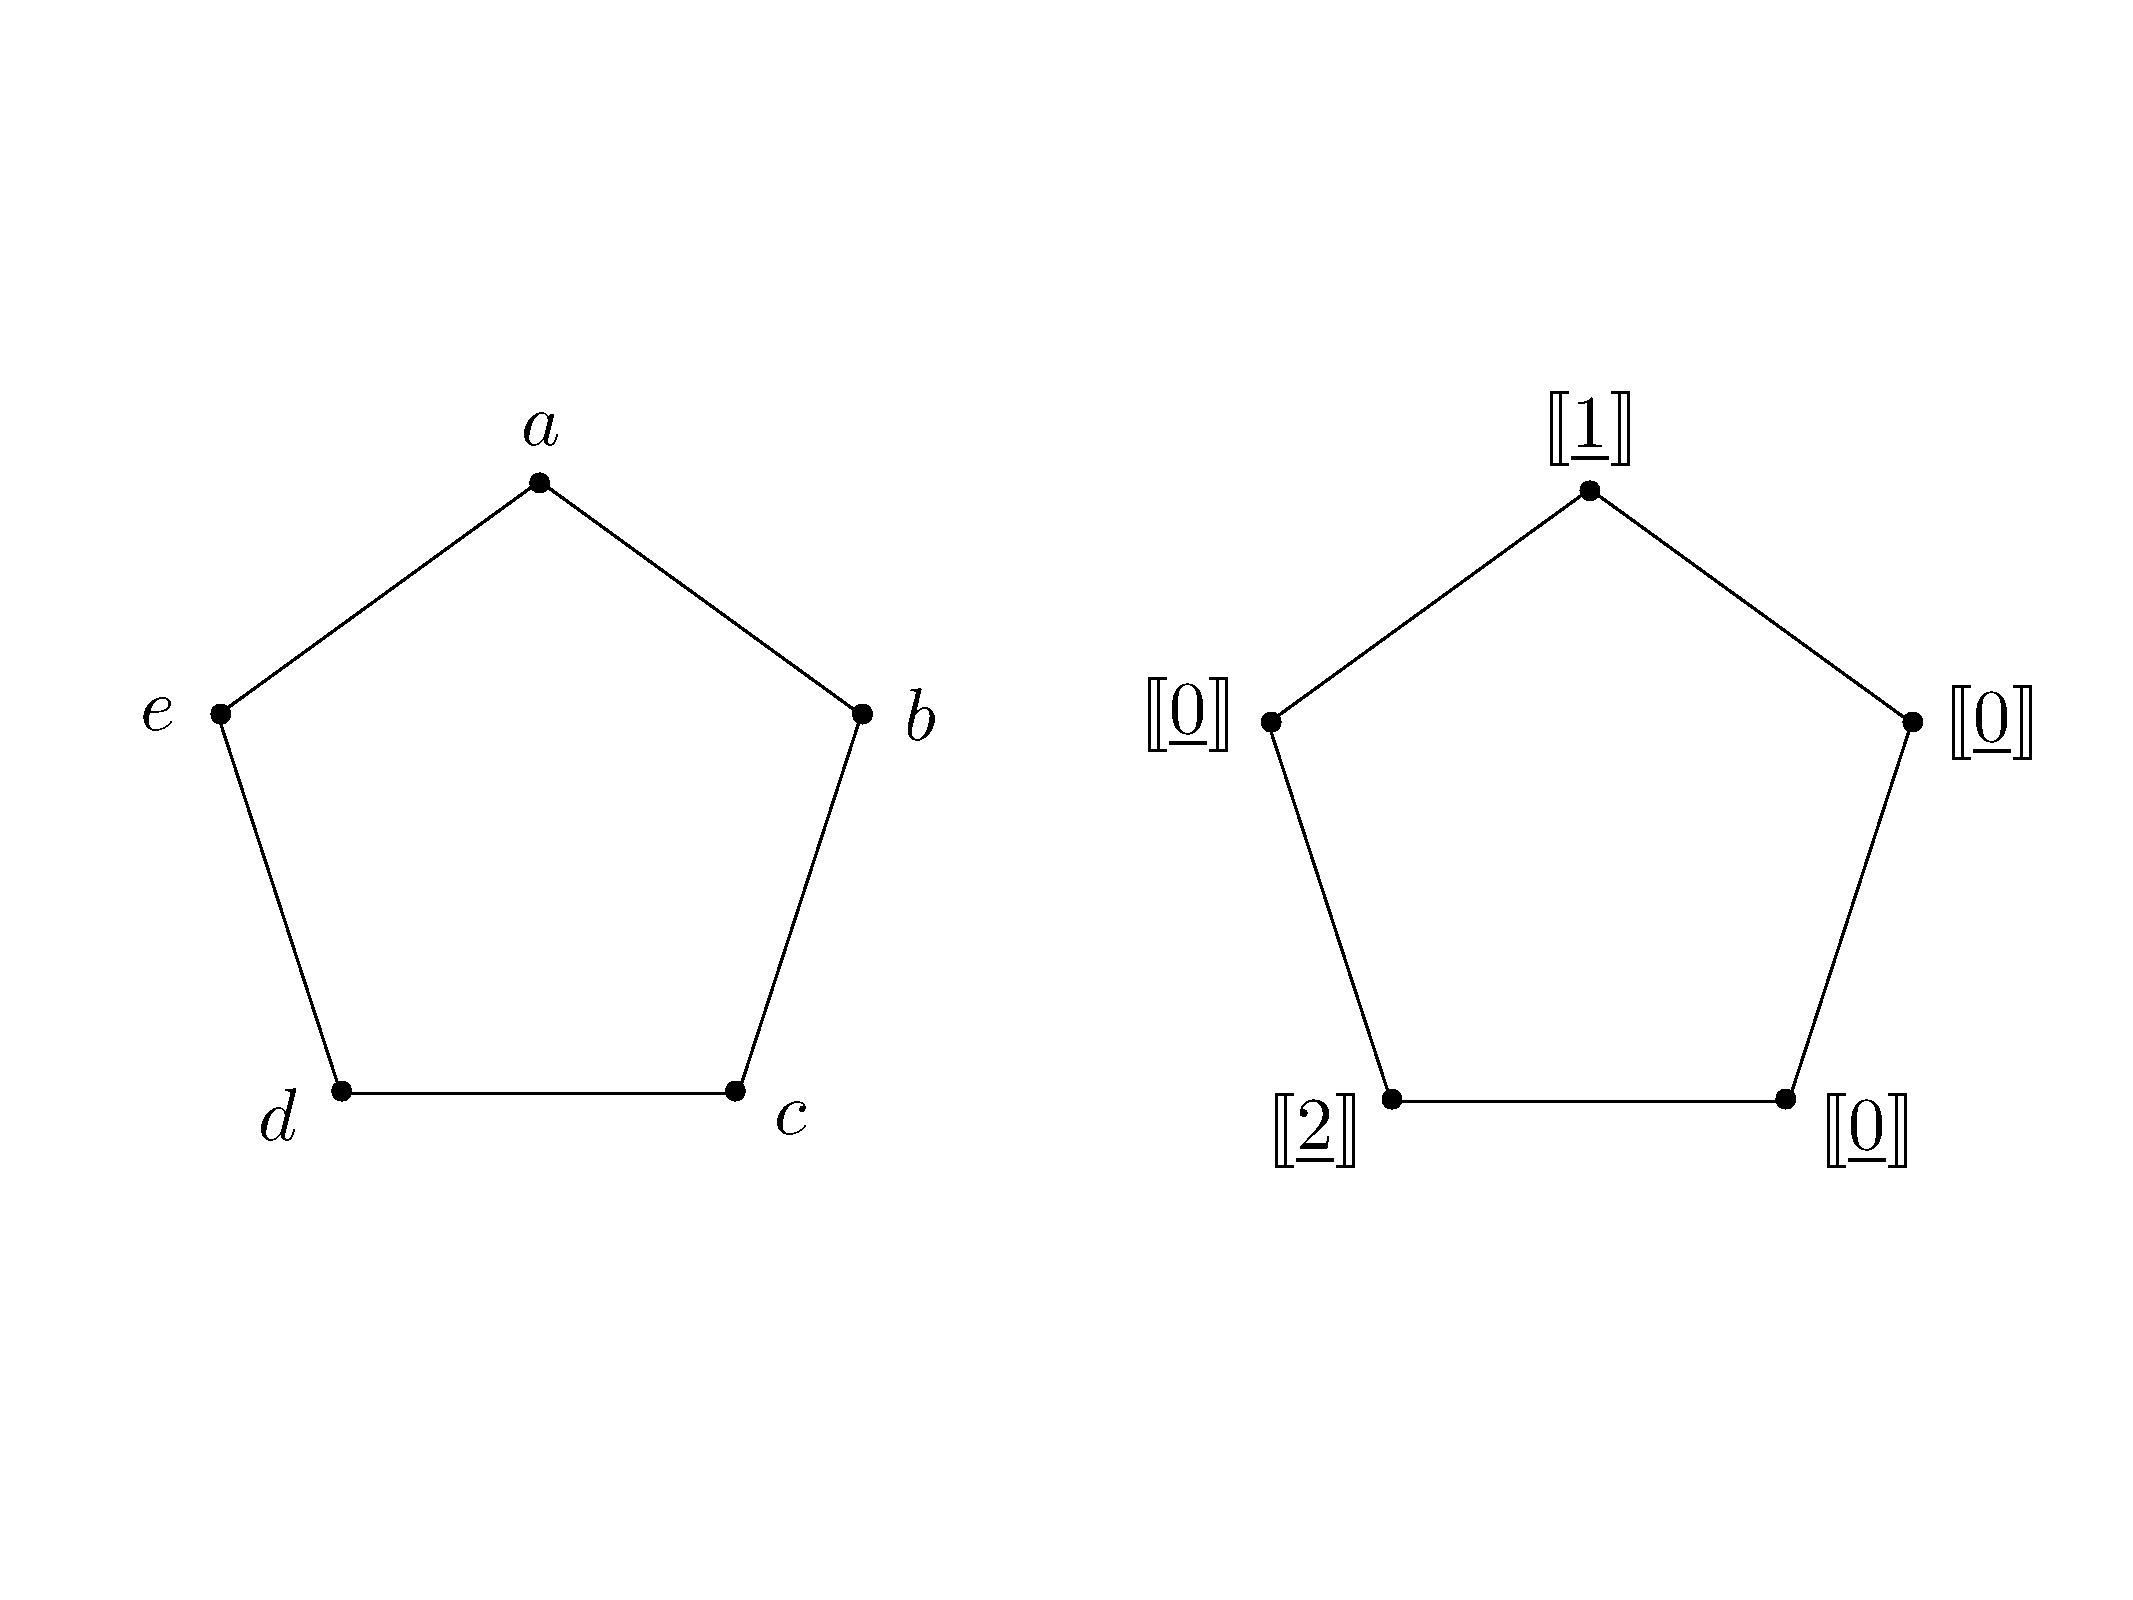
\includegraphics[scale=0.3]{dia2}
\end{center}
We consider a modification of the NTM in which the contents of the second ring control the motion of the read address of the first ring (rather than this being manipulated directly by the RNN controller). To demonstrate the dynamics in an example, suppose that the memory state is as shown at time $t = t_0$, that the read address for the first ring is focused at the zero position at time $t_0 - 1$, and that the read address for the second ring is focused at zero at time $t_0$ and increases its focus position by one step over each time interval. 

Then as time increases from $t_0$ the repeating sequence
\be\label{eq:deliver_iterators}
\den{\underline{1}}, \den{\underline{0}}, \den{\underline{0}}, \den{\underline{0}}, \den{\underline{2}}, \den{\underline{0}}, \ldots
\ee
will be used to control the read address of the first memory ring. More precisely, the operator applied to the read address $r_1 \in \mathscr{W}$ will be $R^n$ with $n$ varying over the repeating sequence $1,0,0,2,0$. Finally, the sequence of vectors delivered to the controller will be
\[
a, b, b, b, d, d, e, e, e, b, \ldots\,.
\]
In more detail, as part of $\master$ there will be an evaluation program
\[
\begin{mathprooftree}
\AxiomC{$\underline{\mathrm{eval}}$}
\noLine\UnaryInfC{$\vdots$}
\def\extraVskip{5pt}
\noLine\UnaryInfC{$\inta_W, {!}(W \multimap W) \vdash W \multimap W$}
\end{mathprooftree}
\]
which has the property that
\[
\den{\underline{\mathrm{eval}}}\big( \sum_i \lambda_i \den{\underline{n}_i}, \ket{\emptyset}_\alpha \big) = \sum_i \lambda_i \alpha^{n_i}\,.
\]
The first argument to this evaluation function will be the state $M_2(r_2) = \sum_i \lambda_i \den{\underline{n}_i}$ of the second memory ring. We apply the output to the read address $r_1$ of the first memory ring and specialise to $\alpha = R$ so that the relevant expression is
\[
\den{\underline{\mathrm{eval}}}( M_2(r_2), \ket{\emptyset}_R )(r_1) = \sum_i \lambda_i R^{n_i}(r_1)\,.
\]
The command and data types are
\begin{gather*}
\Gamma = \inta_{W^{\vee}}, \inta_W, \inta_{W^{\vee}}\,\\
\Delta = W \multimap W, W^{\vee} \multimap W^{\vee}, W \multimap W, W^{\vee} \multimap W^{\vee}, V, \inta_W\,.
\end{gather*}
The first type in $\Gamma$ is connected to the write address for the first memory ring, while the second and third types relate respectively to the read and write address of the second memory ring. We do not include an input to the master algorithm for manipulating the read address of the first memory ring since this is purely under the control of the second memory ring. As usual $\master^z$ is a proof of ${!}\Gamma, {!}\Delta \vdash A \multimap A$. 

Given the command and data vectors
\[
g = \big( \den{\underline{n}_1}, \den{\underline{m}_2}, \den{\underline{n}_2}, \alpha_1, \beta_1, \alpha_2, \beta_2, u_1, u_2 ) \in \bigoplus_{i=1}^3 \mathscr{P}_i \oplus \bigoplus_{j=1}^6 \mathscr{B}_j
\]
and state vector
\[
h = (h_0, r_1, w_1, r_2, w_2, M_1, M_2) \in \mathscr{H} = \mathscr{H}_0 \oplus \mathscr{W} \oplus \mathscr{W}^* \oplus \mathscr{W} \oplus \mathscr{W}^* \oplus \mathscr{S}_1 \oplus \mathscr{S}_2
\]
the value of the master functions are
\[
\den{\master^{\mathrm{in}}}_{nl}(g)(h)
= \big(V(M_1(r_1)), 0, 0, 0, 0, 0, 0 \big)\,.
\]
and
\begin{align*}
\den{\master^{\mathrm{out}}}_{nl}&(g)(h) = \Big( 0, \den{\underline{\mathrm{eval}}}\big( M_2(r_2), \ket{\emptyset}_{\alpha_1} \big)(r_1), \beta_1^{n_1}(w_1),\\
&\qquad \quad \alpha_2^{m_2}(r_2), \beta_2^{n_2}(w_2), M_1 + \beta_1^{n_1}(w_1) \otimes u_1, M_2 + w_2 \otimes u_2 \Big)\,.
\end{align*}
As above we set $\alpha_1 = \alpha_2 = R$ and $\beta_1 = \beta_2 = R^*$. 

\subsection{Multiple pattern NTM}\label{example:ntm_super}

In the previous example the second memory ring stores patterns of memory access in the form of sequences of integers, or more precisely, proofs of linear logic of type $\inta_W$. More complex patterns (this word being of course a euphemism for \emph{algorithms}) can be encoded using more rings and higher types, in various ways.

In this section we give one example, using a pair of additional rings with coefficients in $\den{\inta_W}$ and third additional ring with coefficients in $\den{\binta_W}$. The idea is that the second and third memory rings encode two patterns of memory access, and we allow the controller to switch between the two patterns at any time using the fourth ring. 

If at some time the read address of the second and third rings are focused at positions containing $\den{\underline{m}}, \den{\underline{n}}$ respectively and the read address of the fourth ring is focused at $\den{\underline{S}}$ for some sequence $S \in \{0,1\}^*$ (notation of Example \ref{example_2}) then the read address of the first ring will be acted on by $R^p$ where
\[
p = am + bn
\]
and $a, b$ are the number of times $0,1$ appear in $S$, respectively. Thus whenever we see $\den{\underline{0}}$ on the fourth ring we will follow the pattern on the second ring, and if we see $\den{\underline{1}}$ we will follow the pattern on the third ring. An entry $\den{\underline{00}}$ on the fourth ring will run the pattern on the second ring but with every ``angle of rotation'' doubled. 

The proof that encodes this logic is
\[
\begin{mathprooftree}
\AxiomC{$\underline{\mathrm{feed}}$}
\noLine\UnaryInfC{$\vdots$}
\def\extraVskip{5pt}
\noLine\UnaryInfC{$\inta_W, \inta_W, \binta_W \vdash \inta_W$}
\end{mathprooftree}
\]
with linear lambda term
\begin{align*}
\underline{\mathrm{feed}} &= (\lambda pqra.(\text{copy $a$ as $a',a''$ in}\\
&\qquad\qquad\quad (r \; ((\text{promote $y$ for $x$ in $p$})\; a')\\
&\qquad\qquad\quad\quad ((\text{promote $y'$ for $x'$ in $q$})\; a''))))\,.
\end{align*}
We will not spell out the full model here since it is essentially the same as the one given in the previous section, with the main difference being that the second entry in the tuple defining $\den{\master^{\mathrm{out}}}_{nl}(g)(h)$ now looks like
\be\label{eq:summerevening}
\den{\underline{\mathrm{feed}}}( M_2(r_2), M_3(r_3), M_4(r_4) )_{nl}( R )(r_1)\,.
\ee
To be more concrete, suppose the read address of the fourth ring is sharply focused at a position containing $\den{\underline{S}}$ where $S$ contains $a$ copies of $0$ and $b$ copies of $1$. If the read addresses of the second and third rings give distributions
\[
M_2(r_2) = \sum_i \lambda_i \den{\underline{m}_i}\,, \qquad M_3(r_3) = \sum_j \mu_j \den{\underline{n}_j}
\]
then the term in \eqref{eq:summerevening} is
\[
\Big( \big( \sum_i \lambda_i R^{m_i} \big)^a \big( \sum_j \mu_j R^{n_j} \big)^b \Big)(r_1)\,.
\]
Clearly this can be written as $\sum_p f_p(\lambda, \mu) R^p(r_1)$ for some polynomials $f_p$ in the variables $\{ \lambda_i, \mu_j \}_{i,j}$. The theory of linear logic and its semantics gives a coherent and general way of writing down polynomials, such as $f_p(\lambda, \mu)$, which achieve a given computational idea (in this case, switching between two patterns of memory access) when inserted into the evolution equation of an RNN.
\newpage

%\begin{remark} If we take instead the coefficient vector space of the memory to be $\End_{\mathbb{R}}(\mathscr{H})$ so that we are storing operators rather than vectors, and change the RNN update equation to have the term
%\[
%\big( M^{(t+1)}(r^{(t+1)}) \big)(h_0^{(t)})
%\]
%then the NTM is a generalisation of the higher-order RNN (which is the special case where $\mathscr{W} = \mathbb{R}$, i.e. $N = 1$). Then all the generalisations we have in mind are very sound, conceptually. Test.
%\end{remark}

%\begin{example} If $\Lambda = \{ \underline{1}, \underline{2} \}$ and $\Pi = \{ \underline{010} \}$ then
%\begin{align*}
%Z &= I\big(p_1^{(t)} V(x^{(t)})( Jh^{(t)}) \big) + I\big( p_2^{(t)} V(x^{(t)})^2(J h^{(t)}) \big)\\
%&\qquad + I\Big( q^{(t)}_{010} \big\{ V(x^{(t)}) \circ V(x^{(t+1)}) \circ V(x^{(t)}) \big\}( J h^{(t)}) \Big)\,.
%\end{align*}
%The first summand here is the same as \eqref{eq:new_term_mRNN}, which shows that the linear logic RNN with $\Lambda = \{ \underline{1} \}, \Pi = \emptyset$ and the weight $p^{(t)}_1$ fixed to the identity, is the multiplicative RNN of \cite{sutskever}.
%\end{example}

%\begin{remark} To avoid too many weights and thus slow training, we follow the multiplicative RNN in assuming that $V$ maps inputs to diagonal matrices. But the whole point of adding the ability to call programs from $\Pi$ is that binary integers intertwine $V(x^{(t)})$ and $V(x^{(t+1)})$ in some useful way, which is compromised if these two matrices commute with one another.

%So in practice we have two auxiliary spaces $\mathscr{K}_1,\mathscr{K}_2$ and two sets of weights $V_i,I_i,J_i$. The index $i = 1$ corresponds to $\Lambda$, and $V_1: \mathscr{I} \lto \End_{\mathbb{R}}(\mathscr{K}_1)$ factors through the subspace of matrices diagonal in a chosen basis. The map $V_2$ is not restricted in this way, but to compensate we take $\dim(\mathscr{K}_2) < \dim(\mathscr{K}_1)$.
%\end{remark}

%\begin{remark} If $\mathscr{I} = \mathbb{R}^{n_I}$ and $\mathscr{H} = \mathbb{R}^{n_H}$ then $V \in M_{n_H^2 \times n_I}(\mathbb{R})$. To avoid an explosion of weights due to the large integer $n_H^2$, we can map $\mathscr{I}$ to operators on a subspace of $\mathscr{H}$. This is done by choosing a decomposition $\mathscr{H} = \mathscr{H}_0 \oplus \mathscr{H}_1$ and letting $\rho: \mathscr{H} \lto \mathscr{H}_1, \iota: \mathscr{H}_1 \lto \mathscr{H}$ be respectively be the projection to and inclusion of the subspace $\mathscr{H}_1$. In the evolution equation we use $\iota \den{\lambda_i}( Vx^{(t+1)} )\big( \rho h^{(t)} \big)$ with $\den{\lambda_i}$ now a function $\End_{\mathbb{R}}(\mathscr{H}_1) \lto \End_{\mathbb{R}}(\mathscr{H}_1)$.
%\end{remark}

\begin{remark} A more powerful system would substitute a neural theorem prover along the lines of \cite{alemi,ntp} in place of the libraries of functional programs $\mathscr{P}_i$. At each time step the RNN controller would predict a continuous vector, which when fed into the neural theorem prover as a set of parameters, generates a symbolic program whose denotation is then coupled back into the RNN \cite{tarlow}.
\end{remark}

%\begin{remark} Although intuitionistic linear logic is a weak system in terms of expressive strength the difficulty of training the RNN with polynomial functions of high degree makes it infeasible to make use of even this much strength. It would, however, be very interesting to define differentiable semantics for second-order logic and try to use this to improve the generalisation ability of neural networks.
%\end{remark}

%\begin{remark} Restricting ourselves to the $\textbf{int}_\alpha$ augmentation for the moment, let us discuss what kind of functions $f: \{0,1\}^* \lto \{0,1\}^*$ we would expect that it would be easier for the LLRNN to learn (all other things being equal) compared to an ordinary RNN. The LLRNN has the ability to predict, using its internal state, how many times to iterate the input-derived operator that is to be applied to the hidden state. Thus a function $f$ which, for instance, sends $0$s to $1$ unless they are preceded by a $0$ in which case they go to $0$, should be helped.
%\end{remark}

%Let $\Lambda = (\lambda_1,\ldots,\lambda_l)$ be a sequence of proofs of $\textbf{int}_\alpha$ and let $\Pi = (\pi_1,\ldots,\pi_k)$ be proofs of $\textbf{bint}_\alpha$. When we say that we allow the RNN controller to call this library of functional programs, what we actually mean is that it can predict at each time step diagonal matrices $\{p^{(t)}_\lambda\}_{\lambda \in \Lambda}$ and $\{q^{(t)}_\pi\}_{\pi \in \Pi}$ that determine which programs are used.

%\begin{definition} The \emph{linear logic} RNN coupled to $\Lambda, \Pi$ has weight matrices $H,U,B$ as in the standard RNN, plus new weights $V, P, Q, C, D, I, J$ and an evolution equation:
%\begin{gather*}
%p^{(t+1)}_\lambda = \sigma\big( P_\lambda h^{(t)} + C_\lambda \big)\,,\\
%q^{(t+1)}_\pi = \sigma\big( Q_\pi h^{(t)} + D_\pi \big)\,,\\
%h^{(t+1)} = \sigma\Big( Z + H h^{(t)} + U x^{(t+1)} + B\Big)
%\end{gather*}
%where
%\begin{align*}
%Z &= \sum_{\lambda \in \Lambda} Ip^{(t+1)}_\lambda\den{\lambda}( Vx^{(t+1)} )\big( Jh^{(t)} \big) + \sum_{\pi \in \Pi} Iq^{(t+1)}_\pi\den{\pi}( Vx^{(t)}, Vx^{(t+1)})\big( Jh^{(t)} \big)\,.
%\end{align*}
%The weight matrices $V,I,J$ are interpreted as linear maps as in \eqref{eq:threelinearmaps}. The operators $p^{(t)}_\lambda$ and $q^{(t)}_\pi$ are diagonal matrices in $\End_{\mathbb{R}}(\mathscr{K})$. The outputs $y^{(t)}$ of the linear logic RNN are defined by the same equation \eqref{eq:output_rnn} as before.
%\end{definition}

%Note that the RNN evolution equation for $h^{(t+1)}$ involves both the current input $x^{(t+1)}$ and the previous input $x^{(t)}$. We do this in order to allow the RNN to learn local transformations of an input sequence. % for instance, the transformation of a sequence $a_0 a_1 a_2 a_3 \cdots$ which swaps every pair of symbols, to get $a_1 a_0 a_3 a_2 \cdots$ might use $\den{\underline{10}}$. More complicated transformations could be learned by adapting the equation to a function of $x^{(i)}, \ldots, x^{(t+1)}$ with a more complicated type than $\textbf{bint}_\alpha$.

\begin{remark} In functional programming languages like differential $\lambda$-calculus \cite{difflambda} and differential linear logic \cite{ehrhard-survey} it is possible to differentiate programs with respect to their inputs, even if the programs are higher-order (that is, take functions as input and return them as output). This is a generalisation of automatic differentiation \cite{griewank} which is widely used to compute derivatives of complicated real-valued functions, for example in the backpropagation algorithms of machine learning packages like TensorFlow \cite[\S 4.1]{tensorflow}. The idea is to augment every computation in a code fragment so that derivatives with respect to a chosen variable are computed along with the main result. In TensorFlow this is done by adding special nodes in the dataflow graph.\footnote{See the ``gradients'' method of tensorflow/python/ops/gradients.py in TensorFlow 0.10} The idea of differential $\lambda$-calculus is similar, but more complex \cite{manzyuk}. It would be interesting to explore augmenting the dataflow graph of TensorFlow directly with terms of differential linear logic, in a way that generalises the coupling between semantics and RNNs in this paper.
\end{remark}

%In order to improve the expressive strength of an RNN, that is, allow it to approximate more complex functions from sequences of input symbols to sequences of output symbols, a natural idea is to provide a library of functional programs that can be ``called'' at each time step. The main problem lies in arranging for these programs to be differentiable, so that gradients can be backpropagated through them at training time.
%One natural approach is to have an abstract, symbolic \emph{source} language in which the relevant functional programs can be written, together with a concrete, differentiable \emph{target} category in which the programs can be interpreted. This interpretation should respect the structure of the functional programs: for example, composition or plugging of programs should be interpreted as composition of differentiable maps. The purpose of the source language is to ensure expressive strength, that is, to provide a library of differentiable maps sufficiently rich to encode nontrivial symbolic transformations. The purpose of the target category is to facilitate a straightforward coupling into the RNN.
%A candidate for the source language is linear logic \cite{girard} which has denotational semantics in differentiable maps \cite{ehrhard-survey}. We use the particular semantics developed in \cite{murfet_ll,murfet_coalg,murfetclift}. The second-order RNN encourages us to view symbols as operators on a vector space, and this aligns very well with the intuition provided by linear logic.

%In this section we give a brief sketch of linear logic. A program $\pi$ of type $M$, written $\pi : M$, is built from atomic pieces by rules that we will not explain here. The simplest rule is composition or \emph{plugging}: given programs $M : \alpha \multimap \beta$ and $N: \beta \multimap \gamma$ we have a combined program $N M: \alpha \multimap \gamma$. A program of type ${!} A \multimap B$ takes inputs of type $A$ and returns outputs of type $B$. The same is true of a program of type $A \multimap B$ but in addition it satisfies a \emph{linearity constraint} in that it uses its input \emph{precisely once}. So the ${!}$ connective marks inputs that may be reused freely (or not used at all). All inputs and outputs are themselves programs of the appropriate type.

%\begin{example} A program $\pi$ of type $\textbf{int}_A$ takes an input $M$ of type $A \multimap A$ that may be used non-linearly, and outputs a program of type $A \multimap A$. For each integer $n \ge 0$ there is a program $\underline{n} : \textbf{int}_A$ called the $n$th \emph{Church numeral}, with the property that it maps an input $M$ to the $n$-fold repetition $M^n$. The Church numeral is an \emph{iterator} (something like a \emph{for} loop in imperative programming) which takes a program $M$ and iterates it $n$ times.
%\end{example}

%\begin{example} A program $\pi$ of type $\textbf{bint}_\alpha$ maps an input of type $\alpha \multimap \alpha$ to a program of type $\textbf{int}_\alpha = {!}(\alpha \multimap \alpha) \multimap (\alpha \multimap \alpha)$. So, given two programs $M,N$ of type $\alpha \multimap \alpha$, we can apply the output $\pi(M)$ to $N$, to get a program of type $\pi(M)(N) : \alpha \multimap \alpha$. 

%Given a binary sequence $S \in \{0,1\}^*$ there is a program $\underline{S} : \textbf{bint}_\alpha$ with the property that it maps an input pair $(M,N)$ to the program which intertwines copies of $M,N$ according to $S$. For example, $\underline{01101}$ sends $(M,N)$ to the program $M N N M N$.
%\end{example}

% Like the simply-typed $\lambda$-calculus which it refines, linear logic is a ``higher-order'' functional programming language. It is a rather weak language, but this is not a concern for the present purpose (see Remark \ref{??}).

% A \emph{denotational semantics} of this language selects for each type $A$ some mathematical object $\den{A}$ and for a program of type $A \multimap B$ a transformation $\den{A} \lto \den{B}$ \cite{mellies}. The precise kind of mathematical object, and transformations between them, is determined by the kind of category we take as the target of the semantics. In this paper we use the Sweedler semantics in vector spaces of \cite{murfet_ll,murfet_coalg}. Starting with an atomic type $\alpha$ whose denotation $\den{A} = \mathscr{K}$ is some finite-dimensional vector space over $\mathbb{R}$, we have
% \begin{align*}
%\den{A \multimap A} = \Hom_{\mathbb{R}}( \den{A}, \den{A} ) = \End_{\mathbb{R}}(\mathscr{K})\,.
%\end{align*}



%The idea of the second-order RNN is to view the input and output symbols as linear operators on a vector space $\mathscr{K}$. Linear logic gives us a language in which to create programs, whose denotations are differentiable maps taking linear operators as input and providing linear operators as output. These maps may not themselves be linear, as the above examples show. 

%Let us conclude with an example involving more complicated types:

%\begin{example} There is a program
%\[
%\underline{subst}: \textbf{bint}_\alpha \multimap \Big( {!}\textbf{bint}_\alpha \multimap \big( {!}\textbf{bint}_\alpha \multimap \textbf{bint}_\alpha \big)\Big)
%\]
%which given three input sequences $\underline{S}, \underline{T}, \underline{U}$ uses the pattern of the sequence $S$ to intertwine copies of $T,U$. A program, say $\den{\underline{T}}$, of type $\textbf{bint}_\alpha$ may be ``promoted'' to a program of type ${!} \textbf{bint}_\alpha$, denoted $\ket{\emptyset}_{\den{\underline{T}}}$. Then, for example,
%\[
%\underline{subst}( \underline{010}, [\underline{T}], [\underline{U}] ) = \underline{T \cdot U \cdot T} : \textbf{bint}_\alpha
%\]
%where $\cdot$ means concatenation.
%\end{example}

\appendix

\section{Lambda terms}\label{section:lambda_terms}

In this section we present the linear lambda terms for the master algorithms in some of the earlier examples.

\bibliographystyle{amsalpha}
\providecommand{\bysame}{\leavevmode\hbox to3em{\hrulefill}\thinspace}
\providecommand{\href}[2]{#2}
\begin{thebibliography}{BHLS03}

\bibitem{dnc}
Graves, Alex, et al. "Hybrid computing using a neural network with dynamic external memory." Nature 538.7626 (2016): 471-476.

\bibitem{frege}
G.~Frege, \textsl{Begriffschrift, a formula language, modeled upon that of arithmetic, for pure thought}, (1879). An english translation appears in \textsl{From Frege to G\"odel. A source book in mathematical logic, 1879--1931}, Edited by J.~van Heijenoort, Harvard University Press, 1967.t

\bibitem{blutecon}
R.~Blute, T.~Ehrhard and C.~Tasson, \textsl{A convenient differential category}, arXiv preprint \href{https://arxiv.org/abs/1006.3140}{[arXiv:1006.3140]}, 2010.

\bibitem{sorensen}
M.~H.~S\o rensen and P.~Urzyczyn, \textsl{Lectures on the Curry-Howard isomorphism} (Vol. 149), Elsevier, (2006).

\bibitem{dlnature}
Y.~LeCun, Y.~Bengio and G.~Hinton, \textsl{Deep learning},  Nature, 521(7553), pp.436--444 (2015).

\bibitem{elman}
J.~Elman, \textsl{Finding structure in time}, Cognitive science, 14(2):179–211, 1990.

\bibitem{ntm}
A.~Graves, G.~Wayne and I.~Danihelka, \textsl{Neural turing machines}, arXiv preprint arXiv:1410.5401 (2014).

\bibitem{armmik}
A.~Joulin and T.~Mikolov, \textsl{Inferring algorithmic patterns with stack-augmented recurrent nets}, Advances in Neural Information Processing Systems, 2015.

\bibitem{graves_etal}
A.~Graves, \textsl{Hybrid computing using a neural network with dynamic external memory}, Nature 538.7626 (2016): 471--476.

\bibitem{yuhai}
Y.~Wu, S.~Zhang, Y.~Zhang, Y.~Bengio and R.~R.~Salakhutdinov, \textsl{On multiplicative integration with recurrent neural networks}, In Advances In Neural Information Processing Systems, pp. 2856-2864. 2016.

\bibitem{irsoy}
O.~Irsoy and C.~Cardie, \textsl{Modeling compositionality with multiplicative recurrent neural networks}, arXiv preprint arXiv:1412.6577 (2014).

\bibitem{sutskever}
I.~Sutskever, J.~Martens and G.~E.~Hinton, \textsl{Generating text with recurrent neural networks} Proceedings of the 28th International Conference on Machine Learning (ICML-11). 2011.

\bibitem{sutskever2}
I.~Sutskever, O.~Vinyals and Q.~V.~Le, \textsl{Sequence to sequence learning with neural networks}, Advances in neural information processing systems, 2014.

\bibitem{firstvsecond}
M.~W.~Goudreau, C.~L.~Giles, S.~T.~Chakradhar and D.~Chen, \textsl{First-order versus second-order single-layer recurrent neural networks}, IEEE Transactions on Neural Networks, 5(3), 511--513, 1994.

\bibitem{secondorder}
C.~L.~Giles, D.~Chen, C.~B.~Miller, H.~H.~Chen, G.~Z.~Sun, Y.~C.~Lee, \textsl{Second-order recurrent neural networks for grammatical inference}, In Neural Networks, 1991., IJCNN-91-Seattle International Joint Conference on (Vol. 2, pp. 273-281). IEEE.

\bibitem{highorderrec}
C.~L.~Giles, G.~Z.~Sun, H.~H.~Chen, Y.~C.~Lee, D.~Chen, \textsl{Higher order recurrent networks and grammatical inference}, In NIPS (pp. 380-387) 1989.

\bibitem{pollack}
J.~B.~Pollack, \textsl{The induction of dynamical recognizers}, Machine Learning, 7(2-3), 227-252 (1991). 

\bibitem{murfet_ll}
D.~Murfet, \textsl{Logic and linear algebra: an introduction}, preprint (2014) [arXiv: 1407.2650].

\bibitem{murfet_coalg}
D.~Murfet, \textsl{On Sweedler's cofree cocommutative coalgebra}, J. Pure and Applied Algebra \textbf{219} (2015) 5289--5304.

\bibitem{girard}
J.-Y.~Girard, \textsl{Linear Logic}, Theoretical Computer Science \textbf{50} (1987), 1--102.

\bibitem{joulin}
A.~Joulin and T.~Mikolov, \textsl{Inferring algorithmic patterns with stack-augmented recurrent nets}, Advances in Neural Information Processing Systems, 2015.

\bibitem{grefen}
E.~Grefenstette, et al, \textsl{Learning to transduce with unbounded memory}, Advances in Neural Information Processing Systems, 2015.

\bibitem{weston}
J.~Weston, C.~Sumit and B.~Antoine, \textsl{Memory networks}, preprint (2014) [arXiv:1410.3916].

\bibitem{zaremba2}
W.~Zaremba, et al., \textsl{Learning Simple Algorithms from Examples}, preprint (2015) [arXiv:1511.07275].

\bibitem{mellies}
P-A.~Melli\`{e}s, \textsl{Categorical semantics of linear logic}, in : Interactive models of computation and program behaviour, Panoramas et Synth\`{e}ses $27$, Soci\'{e}t\'{e} Math\'{e}matique de France, 2009.

\bibitem{alemi}
A.~A.~Alemi, F.~Chollet, G.~Irving, C.~Szegedy and J.~Urban, \textsl{DeepMath-Deep Sequence Models for Premise Selection}, arXiv preprint arXiv:1606.04442.

\bibitem{tarlow}
M.~Balog, A.~L.~Gaunt, M.~Brockschmidt, S.~Nowozin and D.~Tarlow, \textsl{DeepCoder: Learning to Write Programs}, arXiv preprint arXiv:1611.01989.

\bibitem{ntp}
T.~Rockt\"aschel and S.~Riedel, \textsl{Learning Knowledge Base Inference with Neural Theorem Provers}, In NAACL Workshop on Automated Knowledge Base Construction (AKBC) 2016.

\bibitem{ehrhard-survey}
T.~Ehrhard, \textsl{An introduction to Differential Linear Logic: proof-nets, models and antiderivatives}, \href{https://arxiv.org/abs/1606.01642}{[arXiv:1606.01642]} (2016).

\bibitem{murfetclift}
J.~Clift and D.~Murfet, \textsl{Cofree coalgebras and differential linear logic}, preprint.

\bibitem{tensorflow}
Abadi, Martín, et al. \textsl{TensorFlow: A system for large-scale machine learning} arXiv preprint arXiv:1605.08695 (2016).

\bibitem{tensorflow2}
Abadi, Martın, et al. \textsl{Tensorflow: Large-scale machine learning on heterogeneous distributed systems}, arXiv preprint arXiv:1603.04467 (2016).

\bibitem{griewank}
A.~Griewank and A.~Walther, \textsl{Evaluating derivatives: principles and techniques of algorithmic differentiation}, Siam (2008).

\bibitem{difflambda}
T.~Ehrhard and L.~Regnier, \textsl{The differential $\lambda$-calculus}, Theoretical Computer Science 309, pp. 1--41, (2003).

\bibitem{manzyuk}
O.~Manzyuk, \textsl{A simply typed $\lambda$-calculus of forward automatic differentiation}, In Mathematical Foundations of Programming Semantics Twenty-eighth Annual Conference, pages 259--73, Bath, UK, June 6–9 2012. \href{http://dauns.math.tulane.edu/~mfps/mfps28proc.pdf}{[URL]}.

\bibitem{minsky}
M.~Minsky, \textsl{Logical versus analogical or symbolic versus connectionist or neat versus scruffy}, AI magazine, 12(2), 34 (1991).

\bibitem{prooftypes}
J.-Y.~Girard, Y.~Lafont and P.~Taylor, \textsl{Proofs and Types}, Cambridge Tracts in Theoretical Computer Science 7, Cambridge University Press, 1989.

\bibitem{benton_etal}
N.~Benton, G.~Bierman, V.~de Paiva and M.~Hyland, \textsl{Term assignment for intuitionistic linear logic}, Technical report 262, Computer Laboratory, University of Cambridge, 1992.

\end{thebibliography}

\end{document}

\section{Old stuff}

The operation to be performed is given by a sequence of vectors
\be\label{eq:weight_P}
p^{(t)}_i = \sigma( P_i h^{(t-1)} ) \in \mathbb{R}^{n_P}\,, 1 \le i \le m
\ee
in a way that we will now explain. In outline, we think of the entries of $p^{(t)}_i$ as telling us the coefficients of monomials in the entries of $x^{(t)}$ and $h^{(t-1)}$ to use in the modified update equation. For simplicity let us only consider monomials of degree $2$ in what follows, since the general case is similar. We set
\be\label{eq:weight_E}
y^{(t)} = E x^{(t)} \oplus h^{(t-1)} \in \mathbb{R}^{n_Y}
\ee
where $E$ is another matrix of weights. See Example \ref{??} for an explanation.

Let $F$ denote a linear map $F: M_{n_Y}(\mathbb{R}) \lto \mathbb{R}^{n_Y^2}$ which reads off the entries of a matrix into a column vector. In TensorFlow we can represent this using \emph{reshape}. Writing $Y = y^{(t)}$ observe that $Y Y^T$ is an $n_Y \times n_Y$ matrix with $(i,j)$-entry $Y_i Y_j$. We choose $n_P = n_Y^2$ and compute the entry-wise multiplication
\[
p^{(t)}_i \odot F(Y Y^T) = p^{(t)}_i \odot F\big( y^{(t)} ( y^{(t)} )^T \big) \in \mathbb{R}^{n_P}\,.
\]
Finally, $q^{(t)}$ is the column vector whose $i$th row is $p^{(t)}_i \odot F(Y Y^T)$, that is,
\[
q^{(t)} = \begin{pmatrix} p^{(t)}_1 \odot F\big( y^{(t)} ( y^{(t)} )^T \big) \\
\vdots\\
p^{(t)}_m \odot F\big( y^{(t)} ( y^{(t)} )^T \big) \end{pmatrix}\,.
\] 
In summary, we view $x^{(t)}, h^{(t-1)}$ as respectively the differentiable analogues of \verb+A,R2+ and the sequence $p^{(t)}_1, \ldots, p^{(t)}_m$ as the analogue of the command \verb+ADD+. The output of the command is the vector $q^{(t)}$. We incorporate this output into the update equation as follows:
\be\label{eq:final_update}
h^{(t+1)} = \sigma\big( V q^{(t)} + H h^{(t)} + U x^{(t+1)} \big)\,.
\ee
Thus $V$ is the differentiable analogue of the register \verb+R3+. The weights are $P_i$ from \eqref{eq:weight_P}, $E$ from \eqref{eq:weight_E} and $V, H, U$ from \eqref{eq:final_update}. This architecture is easily generalised to polynomials of higher degree, by adding additional terms.

\begin{example} Let us consider how the system might reproduce the program that repeats every digit of an input binary sequence, e.g.
\be\label{eq:approx_map}
0110 \longmapsto 00111100\,.
\ee
We take the inputs $x \in \mathbb{R}^2$ with $e_1 = (1,0)$ standing for the binary digit $1$ and $e_0 = (0,1)$ standing for $0$. We suppose that the system has learned the embedding matrix $E$ such that $A = E(e_1)$ and $B = E(e_0)$ are matrices in $M_n(\mathbb{R}_{>0})$ with the property that the subgroup they generate under multiplication is a free group on two letters. This condition just means that the map
\[
\Psi: \{0,1\}^* \lto M_n( \mathbb{R} )
\]
from binary sequences to matrices, defined inductively for $s \in \{0,1\}$ by
\[
\Psi( s S ) = \begin{cases} B \Psi(S) & s = 0 \\ A \Psi(S) & s = 1 \end{cases}
\]
is injective. The space of matrices $\mathscr{H} = M_n(\mathbb{R})$ is the internal state of our RNN. To extract output from the RNN we apply a series of fully-connected layers with the final internal state $h^{(T)}$ as input, and we think of this series of layers as approximating a function $\Psi': M_n(\mathbb{R}) \lto \{0,1\}^*$ with the property that $\Psi' \circ \Psi = 1$, that is, which can read off from a product of matrices $ABA$ the corresponding binary sequence $101$. So, in order to approximate the function \eqref{eq:approx_map} our RNN needs to take the inputs
\[
x^{(1)} = B, x^{(2)} = A, x^{(3)} = A, x^{(4)} = B
\]
and produce the final internal state
\[
h^{(T)} = BBAAAABB \in M_n(\mathbb{R})\,.
\]
This can be be done if we assume that in the update equation \eqref{eq:final_update} has weights $H, U = 0$ and $V$ is chosen so that
\[
V q^{(t)} = (x^{(t)})^2 h^{(t-1)}\,.
\]
Note that the right hand side is a cubic polynomial in the entries of $x^{(t)}, h^{(t-1)}$ so we actually need the generalised form of \eqref{eq:final_update}.
\end{example}

\begin{example}[(Stack-augmented RNN)] Thinking of an RNN as a state machine automata, and by analogy with a pushdown automata, an RNN can be augmented with an external stack memory \cite{highorderrec}. We can emulate the more recent version of this idea in \cite{joulin} with appropriate choices of the defining data of the LLRNN. We begin with a decomposition of the hidden state space as $\mathscr{H} = \mathscr{H}_0 \oplus \mathscr{S}$ where the ``memory stack''
\be
\mathscr{S} = k[z]/z^{N+1} = k1 \oplus kz \oplus \cdots \oplus kz^N
\ee
is equipped with the push and pop operators $p_{+},p_{-}: \mathscr{S} \lto \mathscr{S}$ with matrices
\[
p_{+} = \begin{pmatrix} 0 & 0 & \cdots & 0 & 0 \\
1 & 0 & \cdots & 0 & 0 \\
0 & 1 & \cdots & 0 & 0\\
\vdots & & \ddots & & \vdots \\
0 & 0 & \cdots & 1 & 0\\
\end{pmatrix}\,,\qquad
p_{-} = \begin{pmatrix} 0 & 1 & 0 & \cdots & 0 \\
0 & 0 & 1 & \cdots & 0 \\
\vdots &  &  & \ddots & \vdots \\
0 & 0 & 0 & \cdots & 1\\
0 & 0 & 0 & \cdots & 0
\end{pmatrix}\,.
\]
We also constrain the weight matrix $H$ to be of the form
\[
H = \begin{pmatrix} H_0 & 0 \\ 0 & 0 \end{pmatrix}
\]
with respect to the direct sum decomposition $\mathscr{H} = \mathscr{H}_0 \oplus \mathscr{S}$. 

The master program is a proof (which we omit) of
\be
{!}1, \,{!}( \inta_A \oplus \inta_A ), \,{!}(S \multimap S), \,{!}(S \multimap S) \vdash A \multimap A
\ee
with the property that $\den{S} = \mathscr{S}$ and
\[
\den{\master}_{nl}(\tau, \den{\underline{m}} \oplus \den{\underline{n}}, \alpha, \beta ) = \tau J(1) + J \circ \alpha^m \circ \beta^n \circ I\,,
\]
where $I: \mathscr{H} \lto \mathscr{S}$ and $J: \mathscr{S} \lto \mathscr{H}$ are the projections and injections respectively. We note that for $\lambda, \mu \in k$
\[
\den{\master}_{nl}( \tau, \lambda\den{\underline{1}} \oplus \den{\underline{0}} + \mu \den{\underline{0}} \oplus \den{\underline{1}}, \alpha, \beta ) = \tau J(1) + \lambda J \circ \alpha \circ I + \mu J \circ \beta \circ I\,.
\]
The command types are $P_1 = 1, P_2 = \inta_A \oplus \inta_A$ and the input types are $B_1 = B_2 = S$. We take $\mathscr{B}_j = \End_{\mathbb{R}}(\mathscr{S})$ for $j \in \{1,2\}$, $\mathscr{P}_1 = k$ and
\be
\mathscr{P}_2 = \operatorname{span}( \den{\underline{1}} \oplus \den{\underline{0}}, \den{\underline{0}} \oplus \den{\underline{1}} ) \subseteq \den{\inta_A} \oplus \den{\inta_A}\,.
\ee
We assume the weight matrices $V_j$ are fixed during training with the image of every basis element equal to $p_{+}$ for $j = 1$ and $p_{-}$ for $j = 2$. 

Now let us explain why this emulates a stack-based memory. At time $t$, we write
\[
h^{(t)} = (h_0^{(t)}, s^{(t)})^T
\]
and view $h_0^{(t)}$ as the internal state of the RNN and $s^{(t)} = (s_0^{(t)}, \ldots, s_N^{(t)})^T$ as the contents of the stack at time $t$. Suppose that the command vectors generated by the controller are the scalar $W_1(h^{(t)}) \in k$ and
\[
W_2(h^{(t)}) = \lambda \den{\underline{1}} \oplus \den{\underline{0}} + \mu \den{\underline{0}} \oplus \den{\underline{1}}
\]
for some $\lambda,\mu \in k$.
Then with $\alpha = p_{+}$ and $\beta = p_{-}$ and  we have
\begin{align*}
H h^{(t)} + Z &= J\den{\master}_{nl}\big( W_1(h^{(t)}), W_2(h^{(t)}), p_+, p_-\big)I( h^{(t)} )\\
&= H h^{(t)} + W_1(h^{(t)}) J(1) + J\big( \lambda p_+ + \mu p_{-} \big)I( h_0^{(t)}, s^{(t)})^T\\
&= H h^{(t)} + J\begin{pmatrix} W_1(h^{(t)}) + \mu s_1^{(t)}, & \lambda s_0^{(t)} + \mu s_2^{(t)}, & \cdots, & \lambda s_{N-1}^{(t)} \end{pmatrix}^T\\
&= \begin{pmatrix}
H_0 h_0^{(t)}, &
W_1(h^{(t)}) + \mu s_1^{(t)}, & 
\lambda s_0^{(t)} + \mu s_2^{(t)},
\cdots,\,
\lambda s_{N-1}^{(t)}
\end{pmatrix}
\end{align*}
which agrees with the hidden state of the stack-augmented RNN \cite{joulin} with hidden-to-hidden weight matrix $H_0$, after it has predicted with probability $\lambda$ to push $W_1(h^{(t)})$ onto the stack, and with probability $\mu$ to pop the stack. To store vectors in a vector space $V$ rather than a scalar at each stack position, we simply replace $\mathscr{S}$ by $\mathscr{S} \otimes V$.
\end{example}

\section{Background on CPUs}\label{section:appendix_cpu}

Recall that an assembly program for an ordinary CPU looks like
\begin{verbatim}
LOAD R1, A
ADD R3, R1, R2
STORE C, R3
\end{verbatim}
Where \verb+R1,R2,R3+ stand for the first three registers of the CPU and \verb+A,B,C+ are numbers representing addresses in memory. Thus series of instructions will result in the CPU fetching a number from memory location \verb+A+ and storing it in \verb+R1+, adding this number to a previously stored number in \verb+R2+ with the result being stored in \verb+R3+, and finally writing that register out to the memory address \verb+C+. In the analogy between a CPU and a vanilla RNN we think of the number read from \verb+A+ as the current input $x^{(t)}$ and the previously stored value in \verb+R2+ as (part of) the internal state $h^{(t-1)}$.

Recent work \cite{??,??} on coupling memory to neural networks takes as its starting point the first of the above instructions \verb+LOAD R1, A+ and makes it ``differentiable'' by having the RNN controller predict at time $t$ both the memory address \verb+A+ and the register \verb+R3+ to write to (in this case for example, as a mask on the vector giving the internal state $h^{(t+1)}$). The same differentiable interpretation can be given of the \verb+STORE+ command. This is done by adding suitable terms to the update equation \eqref{eq:update_eqn}.

In contrast our focus is on the third command, the \verb+ADD+. We increase the expressive power of the update equation by allowing it to predict at time $t$ an operation $p^{(t)}$ (a vector specifying a point in a space of ``programs'') which is to be performed on the input and internal state. In order to preserve our analogy with CPU instructions even without \verb+LOAD+ and \verb+STORE+, we could imagine a CPU with a command
\begin{verbatim}
ADD R3, A, R2
\end{verbatim}
which at once reads the number from address \verb+A+, adds it to the stored value in \verb+R2+ and writes the result to \verb+R3+. Note that without a \verb+LOAD+ instruction, the only way a value could have gotten into \verb+R2+ in a previous time step is as the result of another \verb+ADD+.

%\begin{remark} Although the architecture takes some inspiration from normal CPUs, there is an important distinction: on a normal CPU the program is given as a series of instructions prior to the beginning of execution. In contrast, in the model we have described each command is \emph{predicted} at runtime from the current internal state. Perhaps we can understand the process intuitively as follows: we are co-learning a part of $H$, call it $H_0$, which generates some part of the internal state $h^{(1)}_{0}, h^{(2)}_{0}, \ldots$ giving a path through the state space on which the weight matrix $P$ picks out the right program to run at each time step. The overall algorithm is distributed amongst the weights of $H_0$ and $P$.

%This also suggests an alternative algorithm: we do not predict $p^{(t)}$ at each time step, rather we have some fixed number of time steps $T$ and matrices of weights $p^{(1)}, \ldots, p^{(T)}$ which are learned by gradient descent.
%\end{remark}

\subsection{Old example}

We could add further memory rings to manipulate the read or write address of the first two memory rings, but this does not introduce anything essentially new. A more interesting demonstration of the underlying ideas of the coupling to linear logic is given in the next example, which adds two additional memory rings: the first stores constructions of \emph{new iterators from old ones} and the second stores \emph{iterators of these constructions}.

For any type $A$ and $n \ge 0$ there is a Church numeral $\underline{n}_A$ which is a proof of $\inta_A$. We have been omitting the subscript and writing $\underline{n}$ for this proof in the above, but in what follows we will need to sometimes reinstate the subscripts.

Consider memory rings with address space $\mathscr{W}$ and coefficient spaces
\[
\mathscr{V}_3 \subseteq \den{ \inta_{W} \multimap \inta_W }\,, \qquad \mathscr{V}_4 \subseteq \den{ \inta_{\inta_W} }
\]
which are spanned by denotations of linear logic proofs. Proofs of $\inta_W \multimap \inta_W$ construct new iterators from old ones, and since these iterators are naturally identified with integers, we are talking about functions $\mathbb{N} \lto \mathbb{N}$. For example, the proof $\pi_k = \underline{\mathrm{mult}}(k,-)$ of this type \cite[\S 6.1]{murfet_ll} has the property that
\begin{gather*}
\den{\pi_k}: \den{\inta_W} \lto \den{\inta_W}\,,\\
\den{\underline{m}_W} \longmapsto \den{\underline{mk}_W}\,.
\end{gather*}
Proofs of $\inta_{\inta_W}$ are iterators of proofs of the type $\inta_W \multimap \inta_W$. For instance, the proof $\underline{n}_{\inta_W}$ of $\inta_{\inta_W}$ applied to a proof $\rho$ of $\inta_W \multimap \inta_W$ returns this proof iterated $n$ times. In particular, $\underline{n}_{\inta_W}$ applied to $\pi_k$ returns $\pi_{k^n}$ \cite[Example 7.4]{murfet_ll}. The read addresses of these new rings allows the controller to specify that the chosen iterator from the second ring of the extended NTM be modified according to the selected proof in the third ring, and that this modification be iterated the number of times specified by the fourth ring.

Once again, let us first explain the dynamics induced by the additional memory rings with an example. Suppose at time $t = t_0$ the memory state of the first two rings is
\begin{center}
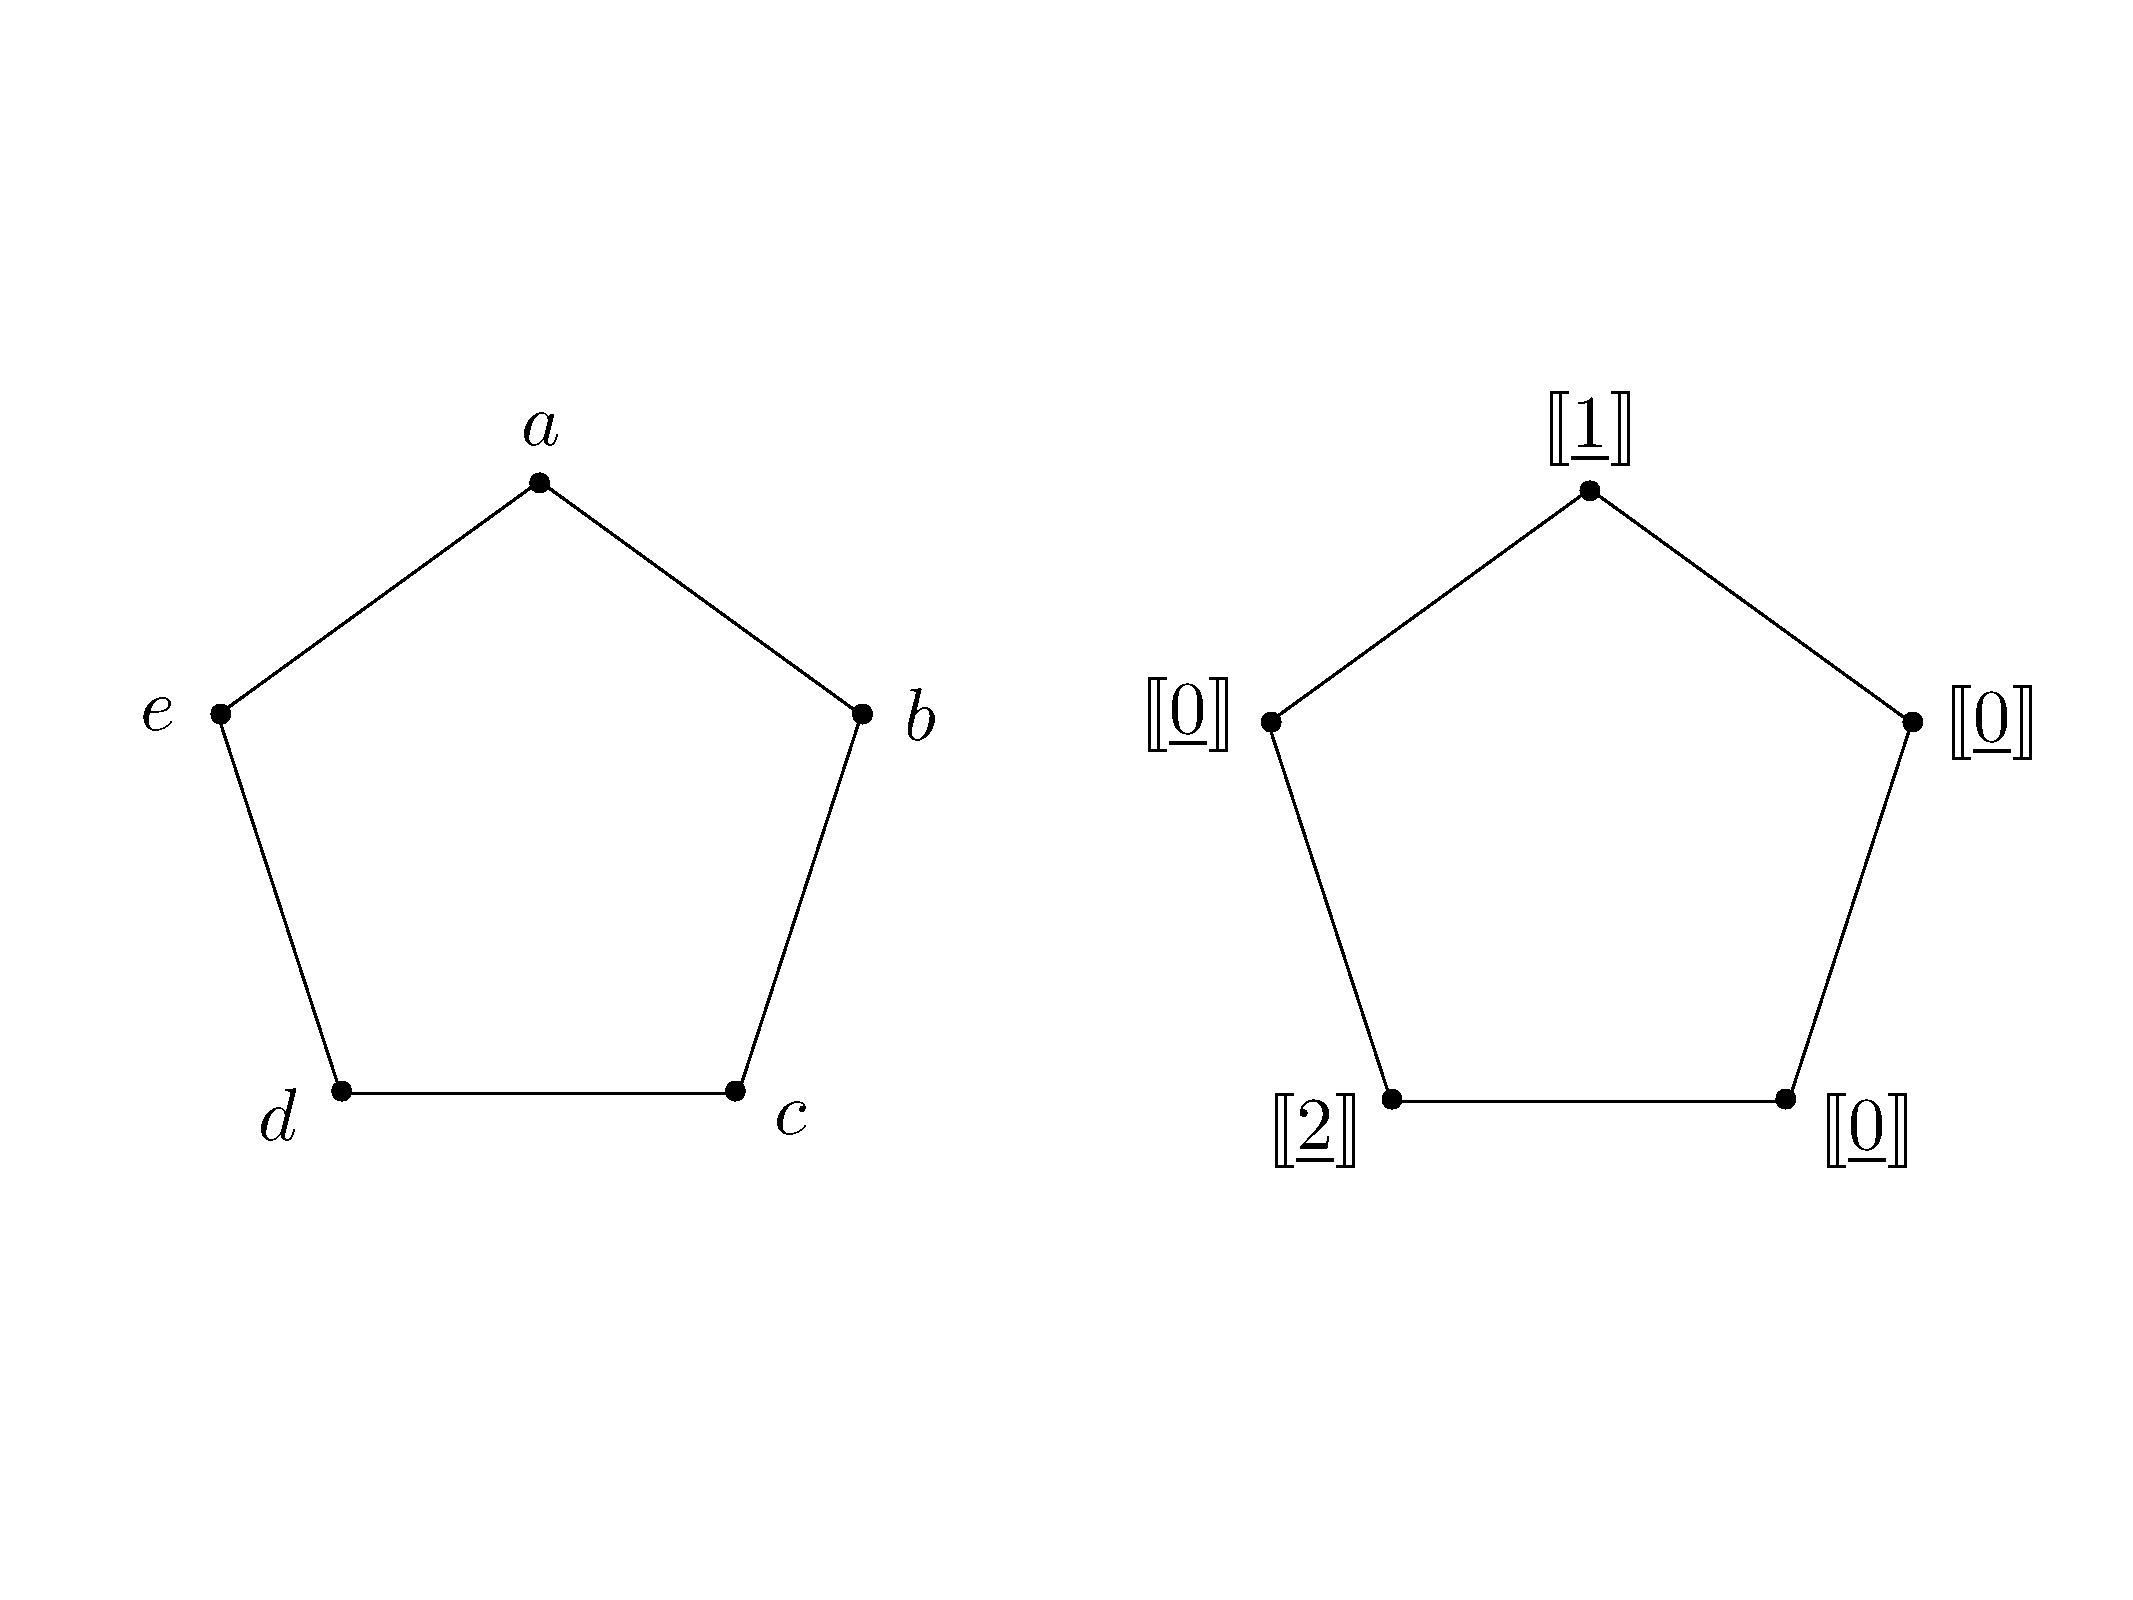
\includegraphics[scale=0.3]{dia2}
\end{center}
and that the state of the third and fourth rings is
\begin{center}
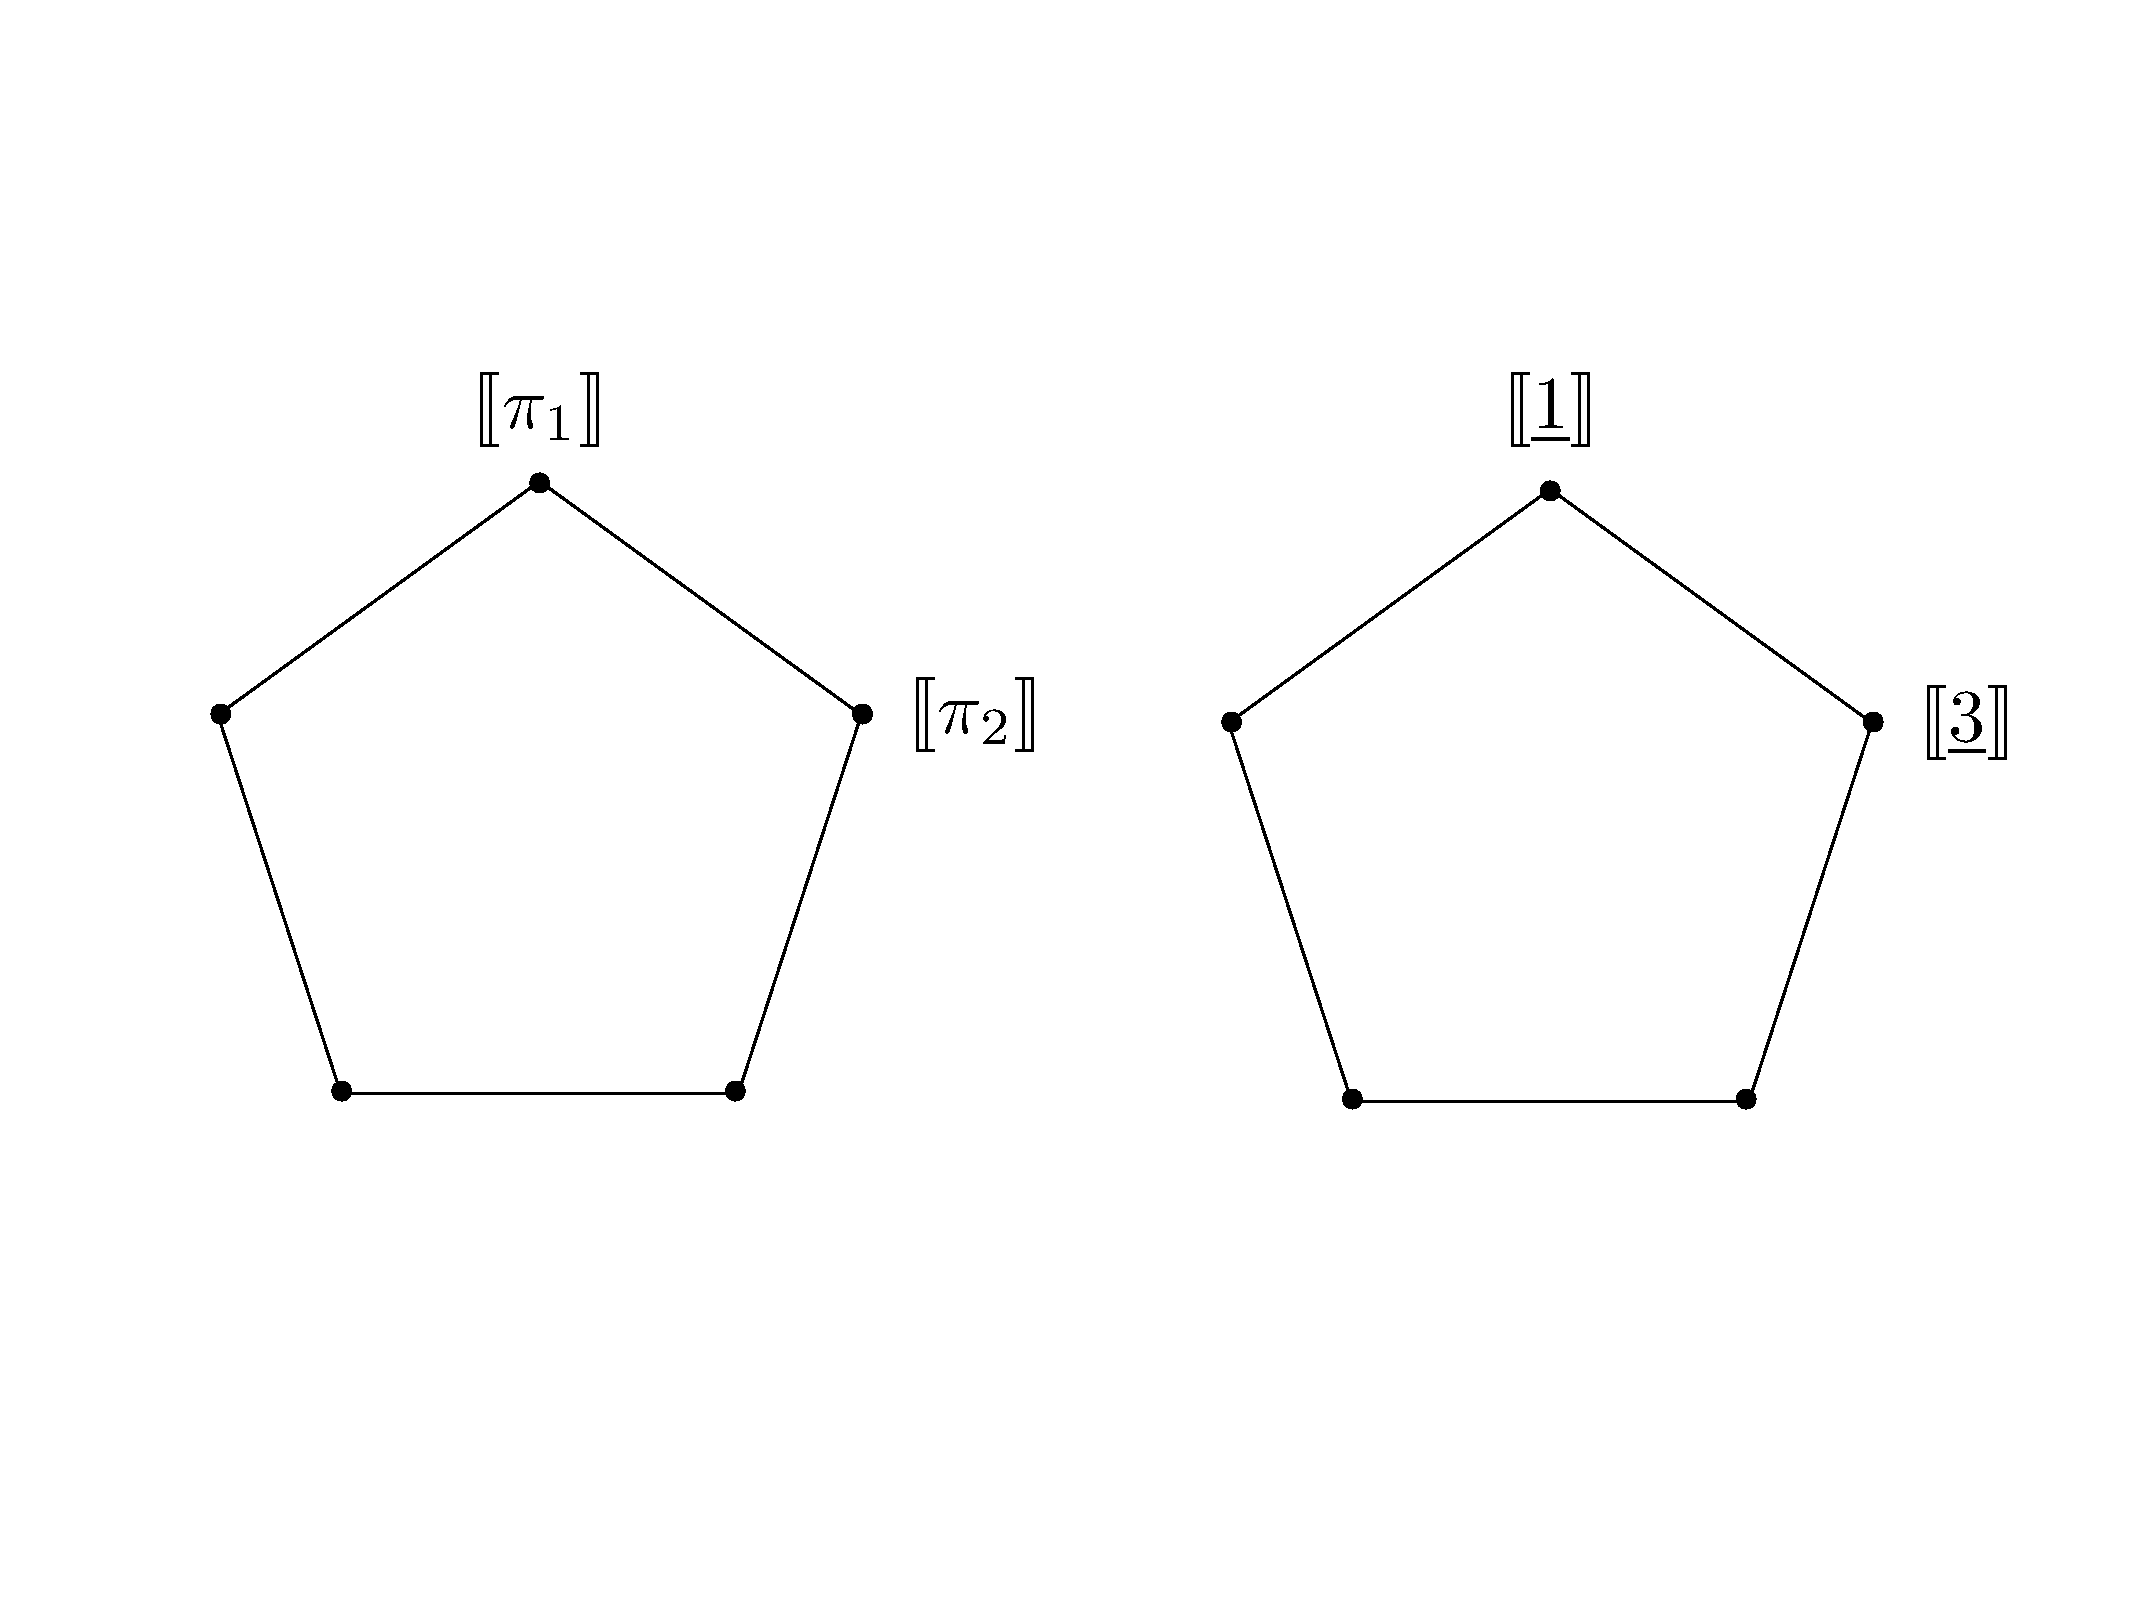
\includegraphics[scale=0.3]{dia3}
\end{center}
Suppose that the read address for the first ring is focused at zero at time $t_0 -1$ and that the focus of the other rings evolves over time according to the table
\begin{center}
\begin{tabular}{|r|c|c|c|c|c|c|c|}
\hline
time after $t_0$ & 0 & 1 & 2 & 3 & 4 & 5 & 6\\
\hline
focus of second ring & 0 & 0 & 1 & 1 & 2 & 1 & 0\\
\hline
focus of third ring & 1 & 0 & 0 & 1 & 1 & 1 & 1\\
\hline
focus of fourth ring & 0 & 0 & 0 & 1 & 0 & 1 & 0\\
\hline
\end{tabular}
\end{center}
At time $t = t_0$ reading from the second, third and fourth rings produces $\den{\underline{2}}, \den{\pi_2}, \den{\underline{1}_{\inta_W}}$ respectively. The controller applies these in reverse order to obtain the iterator
\[
\big\{ \den{\underline{1}_{\inta_W}}( \den{\pi_2} ) \big\}( \den{\underline{2}} ) = \den{\pi_2}( \den{\underline{2}} ) = \den{\underline{4}}\,.
\]
This modified iterator (modified from $\underline{2}$ by the algorithm which is the modification of $\pi_2$ by $\underline{1}_{\inta_W}$) will be the one used by the controller to compute the change in the read address of the first ring from time $t_0 - 1$ to time $t_0$, via the formula
\[
r^{(t_0)} = \den{\underline{4}}_{nl}(R)( r^{(t_0 - 1)} ) = R^4( \overline{0} ) = \overline{4}\,.
\]
This change results in $u_4$ appearing in the computation of $h^{(t_0+1)}$. Using the identity
\begin{gather*}
\big\{\den{\underline{n}_{\inta_W}}_{nl}\big( \den{\pi_k} \big)\big\}\big( \den{\underline{m}_W} \big) = \den{\pi_k}^n( \den{\underline{m}_W} ) = \den{\underline{k^n m}_W}
\end{gather*}
we compute the remaining time steps involve the following iterators:
\begin{align*}
\big\{ \den{\underline{1}_{\inta_W}}_{nl}( \den{\pi_1} ) \big\}( \den{\underline{2}} ) &= \den{\pi_1}( \den{\underline{2}} ) = \den{\underline{2}}\,,\\
\big\{ \den{\underline{1}_{\inta_W}}_{nl}( \den{\pi_1} ) \big\}( \den{\underline{3}} ) &= \den{\pi_1}( \den{\underline{3}} ) = \den{\underline{3}}\,,\\
\big\{ \den{\underline{3}_{\inta_W}}_{nl}( \den{\pi_2} ) \big\}( \den{\underline{3}} ) &= \den{\pi_8}( \den{\underline{3}} ) = \den{\underline{24}}\,,\\
\big\{ \den{\underline{1}_{\inta_W}}_{nl}( \den{\pi_2} ) \big\}( \den{\underline{1}} ) &= \den{\pi_2}( \den{\underline{1}} ) = \den{\underline{2}}\,,\\
\big\{ \den{\underline{3}_{\inta_W}}_{nl}( \den{\pi_2} ) \big\}( \den{\underline{3}} ) &= \den{\pi_8}( \den{\underline{3}} ) = \den{\underline{24}}\,,\\
\big\{ \den{\underline{1}_{\inta_W}}_{nl}( \den{\pi_2} ) \big\}( \den{\underline{2}} ) &= \den{\pi_2}( \den{\underline{2}} ) = \den{\underline{4}}\,.
\end{align*}
The sequence of vectors delivered to the controller will therefore be 
\[
u_0, u_4, u_6 = u_1, u_9 = u_4, u_{33} = u_3, u_{35} = u_0, u_{59} = u_4, u_{63} = u_3.
\]
%When the focus of the fourth ring is at the zero position, the stored proof $\underline{1}_{\inta_W}$ acts on both $\pi_1, \pi_2$ by iterating them once, that is, it does nothing. However, when the focus of the fourth ring is at position one, the stored proof $\underline{3}_{\inta_W}$ at this position iterates any given proof three times, giving respectively $\pi_1, \pi_8$ when fed $\pi_1, \pi_2$. 
Recall that the contents of the second memory ring in the extended NTM appear in the evolution equation via the term $\den{\underline{\mathrm{eval}}}\big( M_2(r_2), \ket{\emptyset}_{\alpha_1} \big)(r_1)$. To define the corresponding term for the current model, we will need the evaluations
\begin{center}
\begin{mathprooftree}
\AxiomC{$\underline{\mathrm{eval}'}$}
\noLine\UnaryInfC{$\vdots$}
\def\extraVskip{5pt}
\noLine\UnaryInfC{$\inta_W \multimap \inta_W, \inta_W \vdash \inta_W$}
\end{mathprooftree}
\qquad
\begin{mathprooftree}
\AxiomC{$\underline{\mathrm{eval}''}$}
\noLine\UnaryInfC{$\vdots$}
\def\extraVskip{5pt}
\noLine\UnaryInfC{$\inta_{\inta_W}, {!}(\inta_W \multimap \inta_W) \vdash \inta_W \multimap \inta_W$}
\end{mathprooftree}
\end{center}
from which we obtain vectors
\begin{gather*}
\den{\underline{\mathrm{eval}}''}( M_4(r_4), \ket{\emptyset}_{M_3(r_3)} ) \in \den{\inta_W \multimap \inta_W}\,,\\
\den{\underline{\mathrm{eval}}'}\Big( \den{\underline{\mathrm{eval}}''}( M_4(r_4), \ket{\emptyset}_{M_3(r_3)} ), M_2(r_2) \Big) \in \den{\inta_W}\,.
\end{gather*}
Since we have four memory rings, the state space of the RNN is decomposed as
\[
\mathscr{H} = \mathscr{H}_0 \oplus \big( \mathscr{W} \oplus \mathscr{W}^* \big)^{\oplus 4}  \oplus \bigoplus_{i=1}^4 \mathscr{S}_i
\]
where $\mathscr{S}_i = \mathscr{W}^* \otimes \mathscr{V}_i$. Using the abbreviations
\[
\Gamma_i = \inta_W, \inta_{W^{\vee}}\,, \qquad \Delta_i = W \multimap W, W^{\vee} \multimap W^{\vee}
\]
the command and data types are given by
\begin{gather*}
\Gamma = \inta_{W^{\vee}}, \Gamma_2, \Gamma_3, \Gamma_4\,\\
\Delta = \Delta_1, \Delta_2, \Delta_3, \Delta_4, V, \inta_W, \inta_W \multimap \inta_W, \inta_{\inta_W}\,.
\end{gather*}
The value of the master function is, for $h = \big(h_0, \{r_i, w_i\}_{i=1}^4, \{M_i\}_{i=1}^4\big)$,
\begin{align*}
\den{\master}_{nl}&\big( \den{\underline{n}_1}, \{\den{\underline{m}_i}, \den{\underline{n}_i}\}_{i=2}^4, \{\alpha_i, \beta_i\}_{i=1}^4, \{u_i\}_{i=1}^4\big)(h)\\
&\quad = \Big(V(M_1(r_1)), \den{\underline{\mathrm{eval}}'}\Big( \den{\underline{\mathrm{eval}}''}( M_4(r_4), \ket{\emptyset}_{M_3(r_3)} ), M_2(r_2) \Big)_{nl}(r_1),\\
&\qquad \beta_1^{n_1}(w_1), \big\{\alpha_i^{m_i}(r_i), \beta_i^{n_i}(w_i)\big\}_{i=2}^4, \big\{M_i + \beta_i^{n_i}(w_i) \otimes u_i \big\}_{i=1}^4 \Big)\,.
\end{align*}
As above we set $\alpha_i = R$ and $\beta_i = R^*$ for $1 \le i \le 4$.